\documentclass{bmstu}
\usepackage{multirow}
\usepackage{graphicx}
\usepackage{hyperref}
\usepackage{subcaption}
\DeclareUnicodeCharacter{0308}{}
\bibliography{biblio}      % Имя вашего .bib файла (без расширения)\textbf{•}

\begin{document}
\makecourseworktitle{Информатика и системы управления}{Программное обеспечение ЭВМ и информационные технологии}{Разработка программы для визуализации оптического преломления через линзы, заданные математическими уравнениями}{ИУ7-52Б}{Ю.~Н.~Городский}{О.~В.~Кузнецова}{}{}

\maketableofcontents

%\include{01-definitions}
%\include{02-abbreviations}

\chapter*{ВВЕДЕНИЕ}
\addcontentsline{toc}{chapter}{ВВЕДЕНИЕ}

	Преломление света — это изменение направления распространения светового пучка при его переходе через границу двух сред с разными показателями преломления. Это явление лежит в основе работы множества оптических приборов, таких как линзы, которые находят широкое применение в фотографии, микроскопии, телескопах и многих других сферах. Классическим примером демонстрации преломления является прохождение света через выпуклую или вогнутую линзу.

	Современные методы моделирования и визуализации позволяют исследовать и воспроизводить это явление с высокой степенью точности. Программное обеспечение для визуализации преломления света через линзы позволяет исследовать и анализировать оптические системы, а так же создавать реалистичные эффекты в кинематографии.

	Целью данной курсовой является разработка программы для визуализации процесса преломления света через аналитически заданные линзы. Программа должна предоставить пользователю возможность выбора источников освещения и объектов, а также параметров сцены для анализа оптических эффектов.

	Для достижения поставленной цели необходимо выполнить следующие задачи:

\begin{itemize} 
	\item[--] изучение явления преломления света и законов оптики с физической точки зрения; 
	\item[--] анализ существующих алгоритмов визуализации оптических эффектов; 
	\item[--] выбор алгоритма для решения поставленной задачи; 
	\item[--] проектирование архитектуры программы и графического интерфейса; 
	\item[--] реализация структур данных и алгоритмов;
	\item[--] описание структуры программного обеспечения; 
	\item[--] реализация программы; 
	\item[--] исследование производительности программы. 
\end{itemize}
\chapter{Аналитическая часть}

	В данном разделе рассмотрены физические основы преломления, существующие алгоритмы построения реалистических изображений и способы хранение трехмерных объектов. Обосновывается выбор алгоритмов и форматов 3д объектов для реализации поставленной задачи. 

	\section{Физическая модель оптических линз}
	Оптическая линза (далее просто линза) - деталь из прозрачного однородного материала, имеющая две преломляющие поверхности, например, обе сферические или же одну плоскую, другую - сферическую.
	Для объяснения физики преломления света при прохождении через оптические линзы, необходимо ввести следующие понятия \cite{1988phs}:
	\begin{itemize}
	\item[--] свет - электромагнитное излучение, распространяемое в виде волны;
	\item[--] поляризованный свет — это свет, в котором направление колебаний вектора напряженности электрического поля упорядочено;
	\item[--] неполяризованный свет - естественный свет, в котором вектор напряженности электрического поля может с равной вероятностью иметь любое направление колебаний в плоскости, перпендикулярной направлению распространения света;
	\item[--] световой луч (луч) -- линия, вдоль которой распространяется световая волна;
	\item[--] фаза луча -- состояние световой волны в момент времени (функция координат и времени);
	\item[--] длина волны -- расстояние между двумя ближайшими друг к другу точками в пространстве, в которых колебания происходят в одинаковой фазе;
	\item[--] абсолютный коэффициент преломления -- безразмерная физическая величина, характеризующая различие фазовых скоростей света в двух средах;
	\item[--] относительный показатель преломления -- безразмерная величина, показывающая отношение абсолютных показателей преломления двух сред.
	\item[--] интенсивность луча -- энергия, переносимая лучом в заданном направлении (от нее зависит яркость излучения).
	\end{itemize}
	
	На рисунке \ref{img/refraction} представлено поведение луча на границе двух сред с разными коэффициентами преломления. Луч, падающий на границу двух веществ, лежит в плоскости чертежа и задан вектором ${k}$, а нормаль к поверхности раздела задана вектором ${n}$. Линия пересечения плоскости падения луча и границы раздела двух сред задана осью $x$, ось $y$ направлена перпендикулярно к плоскости раздела сред. Траектория луча в таком случае представлена на рисунке \ref{img/refraction}.
	
	\begin{figure}[H]
		\center{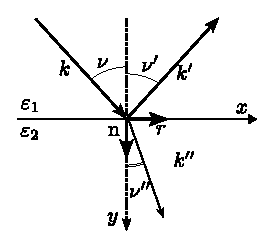
\includegraphics[width=\textwidth, height=50mm, width=170mm, keepaspectratio]{img/refraction.eps}}
		\caption{Траектория луча на границе двух сред}
		\label{img/refraction}
	\end{figure}
	
		Преломленный луч лежит в одной плоскости с падающим лучом и нормалью, востановленной в точке падения. Отношение синуса угла падения к синусу угла преломления есть постоянная величина для заданных веществ.\cite{savelev} При этом углы преломления и отражения задаются уравнениями \ref{eq/refraction_angle} и \ref{eq/reflection_angle} соответвенно.
\begin{equation}
\label{eq/refraction_angle}
n_1 \sin \nu = n_2 \sin \nu ''
\end{equation}
\begin{equation}
\label{eq/reflection_angle}
\nu = \nu'
\end{equation}

Существует два основных коэффициента отражения: для света с параллельной поляризацией ($R_p$) и для света с перпендикулярной поляризацией ($R_s$):
\begin{eqnarray}
\label{eq/FrenelPerp}
R_s = \left( \frac{n_1\cos(\theta_1) - n_2\cos(\theta_2)}{n_1 \cos(\theta_1) + n_2 \cos(\theta_2)} \right)^2\\
\label{eq/FrenelParall}
R_p = \left( \frac{n_2\cos(\theta_1) - n_1\cos(\theta_2)}{n_2 \cos(\theta_1) + n_1 \cos(\theta_2)} \right)^2,
\end{eqnarray}
где:
\begin{itemize}
\item[--] $n_1$ 	и $т_2$ -- показатели преломления первой и второй среды;
\item[--] $\theta_1$ -- угол падения луча на поверхность раздела сред;
\item[--] $\theta_2$ -- угол преломления, который вычисляется по закону \ref{eq/refraction_angle}.
\end{itemize}

Для неполяризованного света коэффициент отражения рас	считывается по формуле:
\begin{equation}
R = \frac{R_s + R_p}{2}
\end{equation}

Коэффициент преломления будет рассчитываться по формуле:
\begin{equation}
T = 1 - R
\end{equation}

При прохождение луча через линзу может наблюдаться явление дисперсии - расхождение световых лучей разного цвета.
    \section{Формализация задачи}
    Формализованная задача представлена на рисунке
    
    	\begin{figure}[H]
		\center{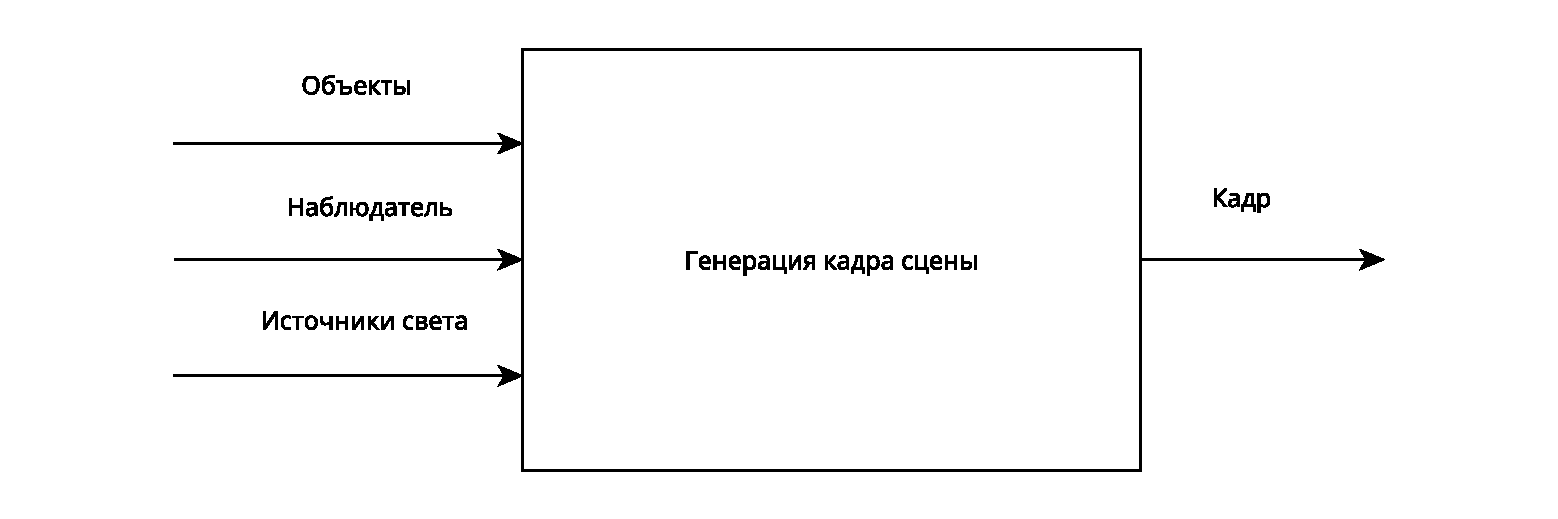
\includegraphics[width=\textwidth, height=1700mm, width=170mm, keepaspectratio]{img/idef0.eps}}
		\caption{Формализованная задача с учетом выбранных алгоритмов}
		\label{img/idef0}
	\end{figure}
	
	\section{Формализация объектов сцены}
	На сцене могут присутствовать следующие типы объектов:
	\begin{itemize}
	\item[--] Сферы с параметрами радиуса, прозрачности, коэффициентом преломления, цветом, уветом излучения и интенсивностью излучения (при излучении света, лучи направлятся в направлении нормали к поверхности сферы);
	\item[--] Линзы с параметрами радиуса, радиуса кривизны, прозрачности, цвета и коэффициента преломления;
	\item[--] Наблюдатель (задается положением, напрвлением зрения и углом обзора);
	\item[--] Полигоны (задаются тремя точками и цветом);
	\end{itemize}
	
	\section{Модель освещения}
	Модель освещения определяет интенсивность освещения $I$ в каждой точке. Наиболее распространенными моделями освеения являются глобальная и лоакльная \cite{leb2011}.
	
	В локальной модели освещения каждый объект рассматривается по отдельности, без учета взаимодействия с другими объектами. Глобальная модель освещения учитывает взаимное расположение объектов. Поскольку для корректного отображения преломления света через линзы необходимо учитывать их взаимное расположение, будет использоваться глобальная модель освещения.
	
	В глобальной модели освещения для каждой точки $P$ пространства сцены интенсивность освещения $I$ будет рассчитываться из 4 состовляющих:
	\begin{itemize}
		\item[--] фоновое освещение, существующее в каждой точке пространства сцены, не зависящее от источников света и координаты точки.
		\item[--] рассеянный свет, распространяющийся равномерно во все стороны, при попадании луча на поверхность объекта, зависящий от ориентации поверхности (нормали $N$ к поверхности в точке), направления на источник света $L$ и интенсивности источника;
		\item[--] зеркальная составляющая, зависящая от зеркальности поверхности и от того, насколько близки направления на наблюдателя и отраженного луча;
		\item[--] преломленная составляющая, зависящая от интенсивности преломленного луча.
	\end{itemize}
	
	Поскольку в задача работы состоит в отображении преломления через лензы, предлагается упростить модель освещения, не учитывая рассеянный свет. В таком случае итоговая составляющая будет рассчитываться по формуле:
	\begin{equation}
	I = k_{\alpha}I_{\alpha} + \sum_j I_j(\overline{N} \cdot \overline{L_j}) + k_{r} I_{r} + k_s I_s
	\end{equation}
	
	где:
	\begin{itemize}
	\item[] $k_{\alpha}$ -- коэффициент фонового освещения;
	\item[] $k_{r}$ -- коэффициент пропускания;
	\item[] $k_s$ -- коэффициент отражения;
	\item[] $I_j$ -- интенсивность j-го источника света;
	\item[] $I_r$ -- интенсивность преломленного луча;
	\item[] $I_s$ -- интенсивность отраженного луча;
	\item[] $\overline{N}$ -- нормаль к поверхности в точке;
	\item[] $\overline{L_j}$ -- вектор, направленный к j-му источнику.
	\end{itemize}
	
	\subsection{Метод фотонных карт}
	Алгоритм создания изображения состоит из трех шагов: на первом шаге испускаются прямые лучи из источников света, распространяются по сцене и формируют распределение фотонов на диффузных поверхностях сцены; на втором шаге на основе полученного распределения фотонов формируются фотонные карты для объектов сцены; на последнем шаге из камеры испускаются обратные лучи и ищется их пересечение с фотонными картами\cite{zhdanov2020}. В точках пересечения с фотонными картами происходит перерасчет светового потока, переносимого фотоном, в яркость вторичного излучения, наблюдаемую в данном направлении:
	     \begin{figure}[H]
		\center{\includegraphics[width=\textwidth, height=70mm, width=170mm, keepaspectratio]{img/photons.png}}
		\caption{Сбор распределения яркости с фотонов при трассировке обратного луча}
		\label{img/photons}
	\end{figure}
	
		\subsection{Простроение освещения с помощью трассировки лучей}
	В алгоритме используется модификация алгоритма, описанного в пункте 1.5.4. Для расчета непрямого освещения для каждой точки дифуззной поверхности при пересечении с лучом трассировки испускается заданное число случайных лучей. После чего они трассируются и на основе их увета формируется непрямое освещение. Такой метод очень трудозатратный, т.к. для количество лучей трассировки резко возрастает.
	

    
    \section{Алгоритмы удаления невидимых поверхностей}

		Удаление невидимых линий и поверхностей заключается в определении тех частей объектов, которые видимы или невидимы для наблюдателя из определенной точки пространства. Эта задача может решаться в двух пространствах:

\begin{itemize}
\item Объектное пространство -- используется физическая система координат, в которой описаны объекты сцены, обеспечивает высокую точность изображения;
\item Пространство изображения -- используется система координат экрана, на котором визуализируется полученное изображение, точность вычислений ограничена разрешающей способностью экрана. 
\end{itemize}
	
	Самыми распространенными алгормами, решающими задачу являются: алгоритм Робертса, z-буффера, трассировки лучей.
        
        \subsection{Алгоритм Робертса}
        Алгоритм Робертса — это один из первых методов для удаления невидимых линий, работающий в объектном пространстве. Он удаляет те ребра и грани, которые скрыты самим объектом\cite{capko2010}. Затем оставшиеся видимые ребра сравниваются с другими объектами для определения, какие их части могут быть скрыты.

	Трудоемкость алгоритма возрастает пропорционально квадрату количества объектов. Он подходит только для работы с выпуклыми телами, а невыпуклые объекты необходимо разбивать на выпуклые части. Поздние версии алгоритма используют предварительную сортировку для повышения эффективности.            

        \subsection{Алгоритм Z--буфера}
        Алгоритм z-буфера — это один из простейших методов удаления невидимых поверхностей в 3D-графике, предложенный Кэтмулом\cite{zbuf2015}. Он работает в пространстве изображения, используя отдельный буфер для хранения глубины каждого видимого пикселя. При отрисовке нового пикселя его глубина сравнивается с той, что уже записана в буфер. Если новый пиксель ближе, он заменяет предыдущий в буфере кадра, и z-буфер обновляется его глубиной. Алгоритм прост, не требует сортировки по глубине, но требует большого объема памяти и может быть менее эффективным при прозрачности или антиалиасинге.

	Пример работы алгоритма, использующего z--буфер, представлен на рисунке \ref{img/z_buffer}.
	
        	\begin{figure}[H]
		\center{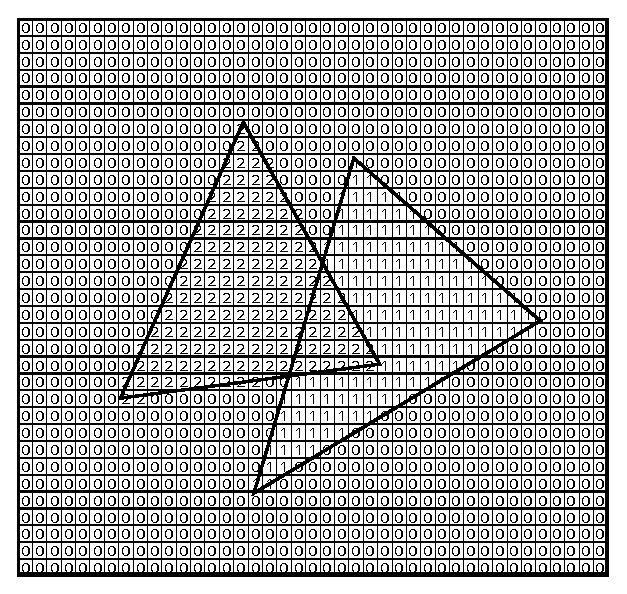
\includegraphics[width=\textwidth, height=130mm, width=170mm, keepaspectratio]{img/z_buffer.eps}}
		\caption{Пример работы алгоритма Z--буфера}
		\label{img/z_buffer}
	\end{figure}
	
		\subsection{Алгоритм Варнока}
        
        Алгоритм Варнока основан на принципе когерентности изображения, при котором большие однородные области требуют меньше усилий для обработки\cite{varnok2017}. Он работает в пространстве изображения и разбивает его на подокна, чтобы определить, простое ли их содержимое. Если содержимое сложное, окно делится дальше, пока не достигнет уровня пиксела. Пример работы алгоритма представлен на рисунке \ref{img/Varnok}.
        
	\begin{figure}[H]
		\center{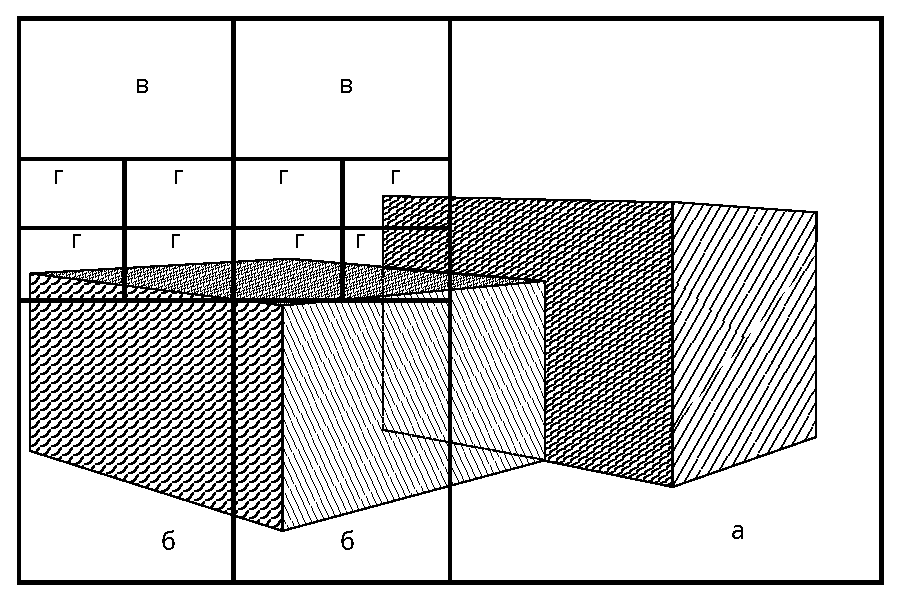
\includegraphics[width=\textwidth, height=70mm, width=170mm, keepaspectratio]{img/Varnok.eps}}
		\caption{Пример работы алгоритма Варнока}
		\label{img/Varnok}
	\end{figure}
        	

Основная идея алгоритма — сосредотачивать вычислительные ресурсы на сложных частях сцены, игнорируя простые области. Метод эффективен для удаления невидимых линий и поверхностей.



                       
        \subsection{Алгоритм обратной трассировки лучей}
        Алгоритм обратной трассировки лучей заключается в том, что для определения видимых поверхностей сцены лучи отправляются от наблюдателя к объекту\cite{backray2006}. Трассировка каждого луча позволяет выяснить, какие объекты сцены пересекаются с данным лучом, учесть преломления, отражения и прохождение сквозь объекты. Пересечения объектов с лучом упорядочиваются по глубине, и ближайшее пересечение указывает на видимую поверхность для каждого пикселя. Пример трассировки лучей представлен на рисунке \ref{img/forward_tras}.
     
     \begin{figure}[H]
		\center{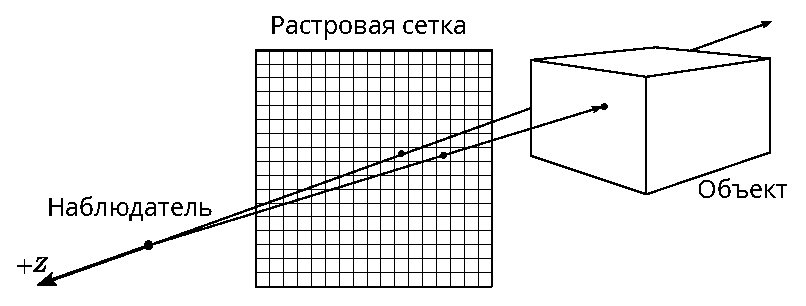
\includegraphics[width=\textwidth, height=70mm, width=170mm, keepaspectratio]{img/forward_tras.eps}}
		\caption{Обратная трассировка лучей}
		\label{img/forward_tras}
	\end{figure}

Основной сложностью алгоритма является определение точек пересечения луча с объектами сцены. Для оптимизации вычислений вводятся габаритные тесты с объемными оболочками (сферами или параллелепипедами) для исключения объектов, с которыми луч не пересекается.

Алгоритм эффективен, если пересечения вычисляются быстро и точно, что существенно влияет на общую производительность. 
                

    
    \section{Способы хранения трехмерных объектов}
   	
   	Классификацию форматов трехмерных бъектов можно провести по 2 параметрам -- это способ описания их геометрии и способ описания их внешнего вида\cite{3f_content_overview}.
   	
   	\subsection{Геометрические параметры 3д объектов}
   		
   	Геометрия моделей часто задаются набором трехмерных точек. Поверхность в таком случае сохраняется ввиде ряда полигонов, которые создаются путем индексации этих вершин. В некоторых форматах используются ребра из 2 вершин. При использовании полигональных моделей для отрисовки круглых объектов можно использовать интерполирование нормалей к каждой грани. При этом существует много вариаций методов интерполирования, наиболее простым из которых является усреднение нормалей, сходящихся в одной вершине, и назначение результата этой вершине. Такой способ хранения 3д объектов достаточен для визуализации 3д контента, где точное определение геометрических свойств не требуется.
   	
   	Для объектов, форму которых можно задать геометрическими примитивами, удобно использовать аналитический способ хранения.
   	   	
   	Другим способом создания 3д моделей является конструктивная твердотельная геометрия. Этот метод использует набор логических операций над геометрическими примитивами. Преимуществом такого метода является точное описание формы объекта, если его так или иначе можно представить набором используемых примитивов, а так же возможность изменить модель на любом этапе ее создания. Данный метод широко используется в САПР.
        
        
    \section{Вывод}

	После оценки вышеизложенных алгоритмов сделан вывод, что для этой работы наиболее подходящим алгоритмом будет алгоритм обратной трассировки лучей, т.к. он позволяет корректно  отобразить симулируемые физические явления, при этом обеспечивая достаточную производительность.
	
Для глобального освещения будет использоваться метод фотонных карт, поскольку он предоставляет возможность моделировать сложные эффекты освещения, такие как мягкие тени, многоступенчатое отражение света и дисперсия, с приемлемым балансом между качеством и производительностью.

	Для хранения линз и сфер будет использоваться аналитический метод(линзы задаются как пересечение двух сфер).
\chapter{Конструкторский раздел}

	В разделе рассмотрены требования к программному обеспечению, схемы алгоритмов, выбранных для решения поставленной задачи. Описаны пользовательские структуры данных, описана структура реализуемого программного обеспчеения.
	
\section{Функциональная модель программного обеспечения}

	Алгоритм получения изображения представлен в виде диаграммы в нотации IDEF0, отражающей также общую структуру программы(рисунок \ref{img/idef0_0} - \ref{img/idef0_2}).
     \begin{figure}[H]
		\center{\includegraphics[width=\textwidth, height=210mm, width=170mm, keepaspectratio]{img/02_A0.png}}
		\caption{Функциональная модель программного обеспечения}
		\label{img/idef0_0}
	\end{figure}
	
	\begin{figure}[H]
		\center{\includegraphics[width=\textwidth, height=210mm, width=170mm, keepaspectratio]{img/03_A2.png}}
		\caption{Функциональная модель построения фотонных карт}
		\label{img/idef0_2}
	\end{figure}
	
	\begin{figure}[H]
		\center{\includegraphics[width=\textwidth, height=210mm, width=170mm, keepaspectratio]{img/04_A4.png}}
		\caption{Функциональная модель трассировки лучей}
		\label{img/idef0_1}
	\end{figure}
	
\section{Используемые типы и структуры данных}
	В программном обеспечении используются следующие типы и структуры данных:
	\begin{enumerate}[label=\textbf{\arabic*.}]
	\item Сцена:
	\begin{itemize}
		\item[--] массив объектов сцены (сферы, линзы, полигоны);
		\item[--] наблюдатель (камера);
		\item[--] фотонная карта прямого освещения;
		\item[--] фотонная карта преломленного и отраженного освещения.
	\end{itemize}
	
	\item Камера:
	\begin{enumerate}
		\item[--] координаты;
		\item[--] вектор направления;
		\item[--] угол зрения.
	\end{enumerate}
	
	\item Сфера:
	\begin{itemize}
		\item[--] радиус;
		\item[--] расположение центра;
		\item[--] графические параметры.
	\end{itemize}
	
	\item Полигон с 3 вершинами:
	\begin{itemize}
		\item[--] 3 вершины;
		\item[--] графические параметры.
	\end{itemize}
	
	\item Линза:
	\begin{enumerate}
		\item[--] расположение центра;
		\item[--] направление центральной оси;
		\item[--] радиус кривизны;
		\item[--] общий радиус линзы (расстояние от центральной оси до края линзы);
		\item[--] графические параметры.
	\end{enumerate}
	
	\item Графические параметры:
	\begin{enumerate}
		\item[--] цвет поверхности;
		\item[--] абсолютный коэффициент преломления;
		\item[--] коэффициент прозрачности;
		\item[--] коэффициент зеркальности;
		\item[--] излучение.
	\end{enumerate}
		\item Излучение
	\begin{enumerate}
		\item[--] цвет;
		\item[--] интесивность.
	\end{enumerate}	
	
	\item Фотон:
	\begin{enumerate}
		\item[--] координаты;
		\item[--] цвет;
		\item[--] направление.
	\end{enumerate}
	
	\item Узел фотонной карты
	\begin{enumerate}
		\item[--] фотон;
		\item[--] указатель на правый узел;
		\item[--] указатель на левый узел.
	\end{enumerate}
	
	\item Фотонная карта
	\begin{enumerate}
		\item[--] указатель на первый узел.
	\end{enumerate}
\end{enumerate}


\section{Формальное описание алгоритмов}
В разделе представлены схемы основных алгоритмов, использующихся в программном обеспечении.
\subsection{Поиск персечения луча и сферы}
на рисунке \ref{img/sphere_intersect} представлен алгоритм поиска пересечения луча с сферой. 
Уравнение сферы можно записать как:
\[
(P - C) \cdot (P - C) = r^2
\]
где $P$ --- точка на поверхности сферы.

Параметрическое уравнение луча задается как:
\[
P(t) = O + t \cdot D
\]
где $t$ --- параметр, определяющий положение точки вдоль луча.


	\begin{figure}[H]
		\center{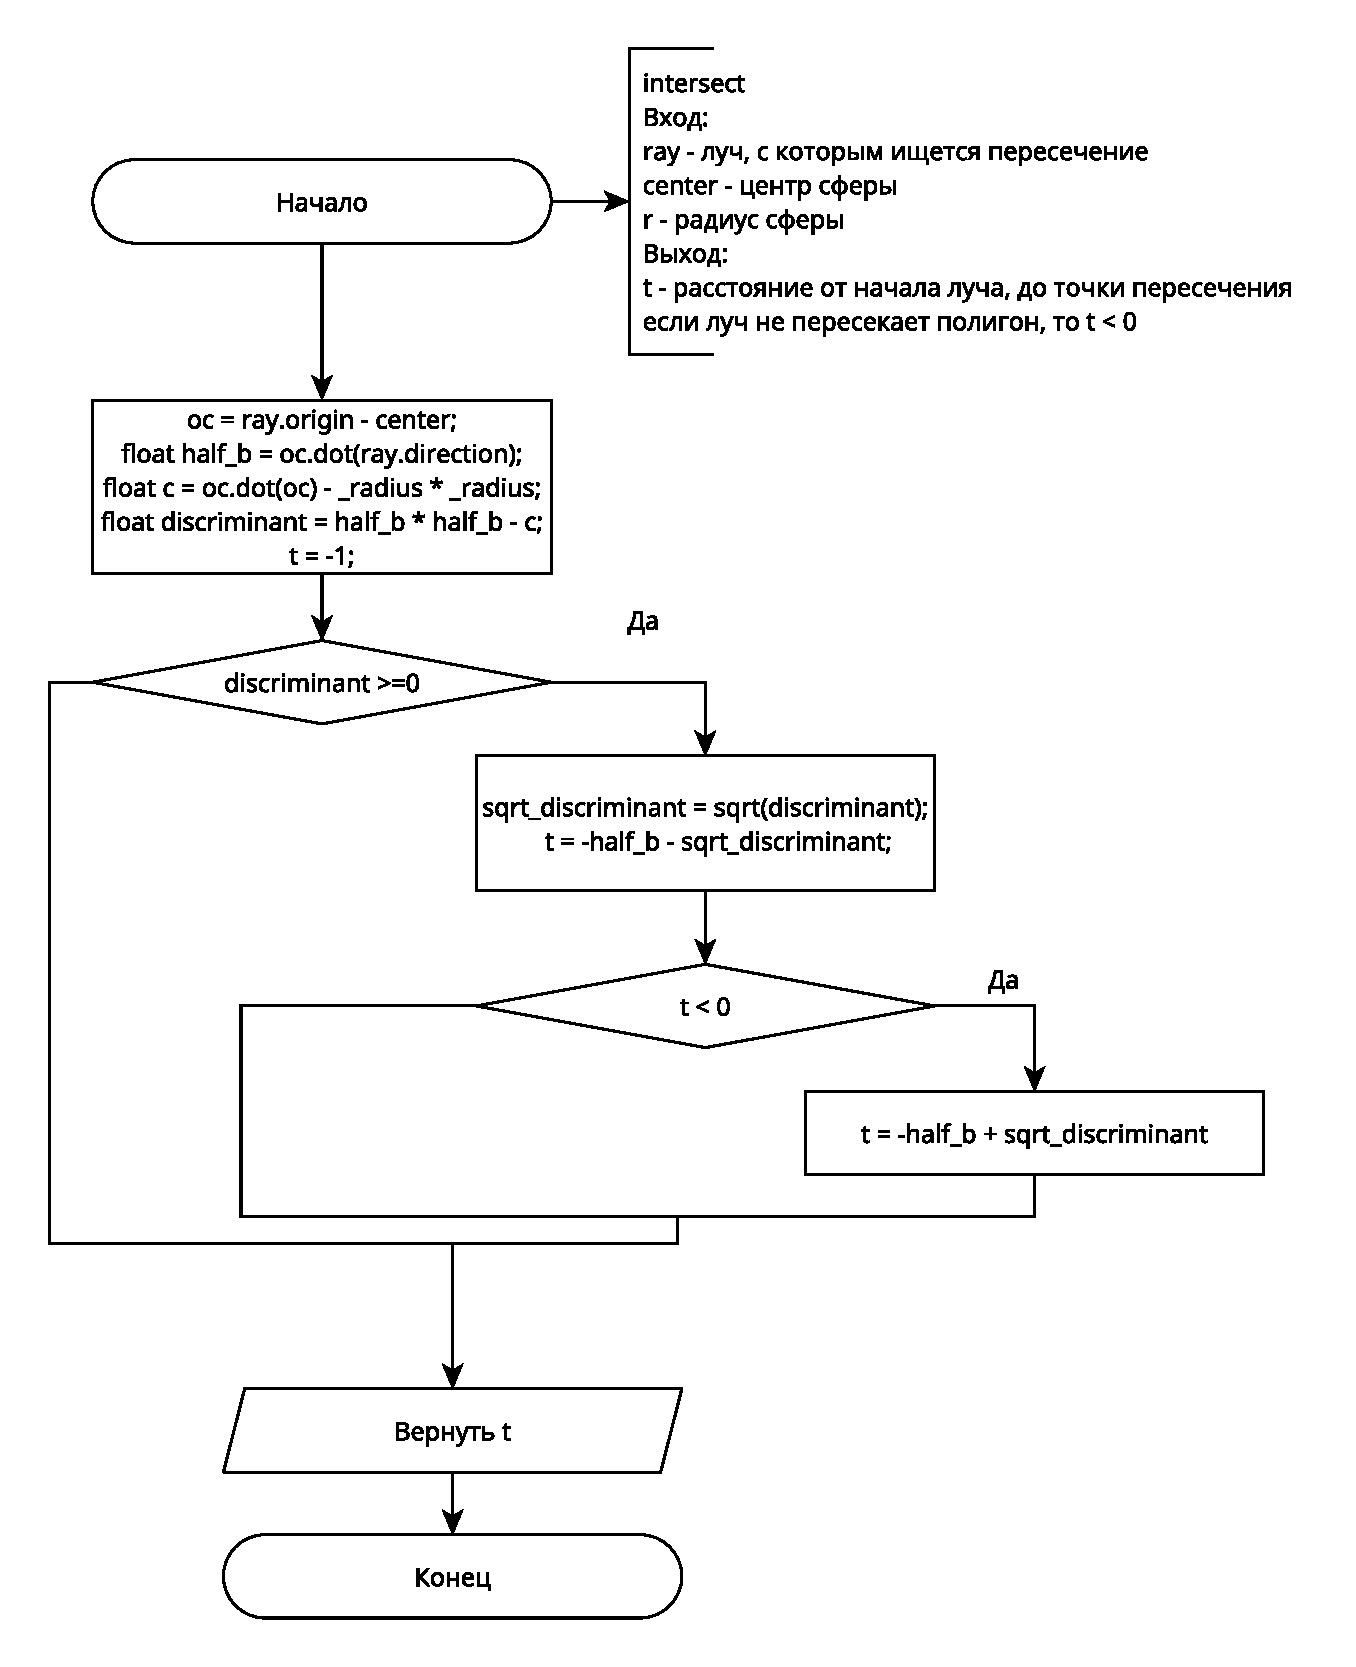
\includegraphics[width=\textwidth, height=210mm, width=170mm, keepaspectratio]{img/sphere_intersect.eps}}
		\caption{Схема алгоритма поиска пересечения с сферой}
		\label{img/sphere_intersect}
	\end{figure}
\subsection{Поиск пересечения луча и полигона}
	Для поиска пересечения луча с треугольным полигоном сначала необходимо проверить, пересекает ли луч плоскость, в которой расположен треугольник. Это можно сделать, проверив, не является ли луч параллельным плоскости, что происходит, если скалярное произведение направления луча и нормали плоскости равно нулю:
\[
(D, n) \neq 0
\]

Если пересечение с плоскостью возможно, вычисляется параметр t, который определяет точку пересечения луча с плоскостью:
\[
t = \frac{(A - V) \cdot n}{(D, n)}
\]
где $A$, $B$ и $C$ — вершины треугольника, $V$ — начальная точка луча, $D$ — направление луча.

Точка пересечения $P$ вычисляется по формуле:
\[
P = V + t \cdot D
\]

После нахождения точки пересечения необходимо проверить, лежит ли она внутри границы треугольника. Для этого задача сводится к двумерному пространству, обнуляя координаты по оси Z у вершин треугольника и точки пересечения.

Затем вычисляются векторные произведения векторов сторон треугольника и векторов, соединяющих первую вершину с точкой пересечения:
\[
v_1 = [AB, AP], \quad v_2 = [BC, BP], \quad v_3 = [CA, CP]
\]

Если все произведения имеют одинаковый знак, то точка пересечения P лежит внутри границы треугольника. Схему алгоритма представлена на рисунке \ref{img/polygon_intersect}
	
	\begin{figure}[H]
		\center{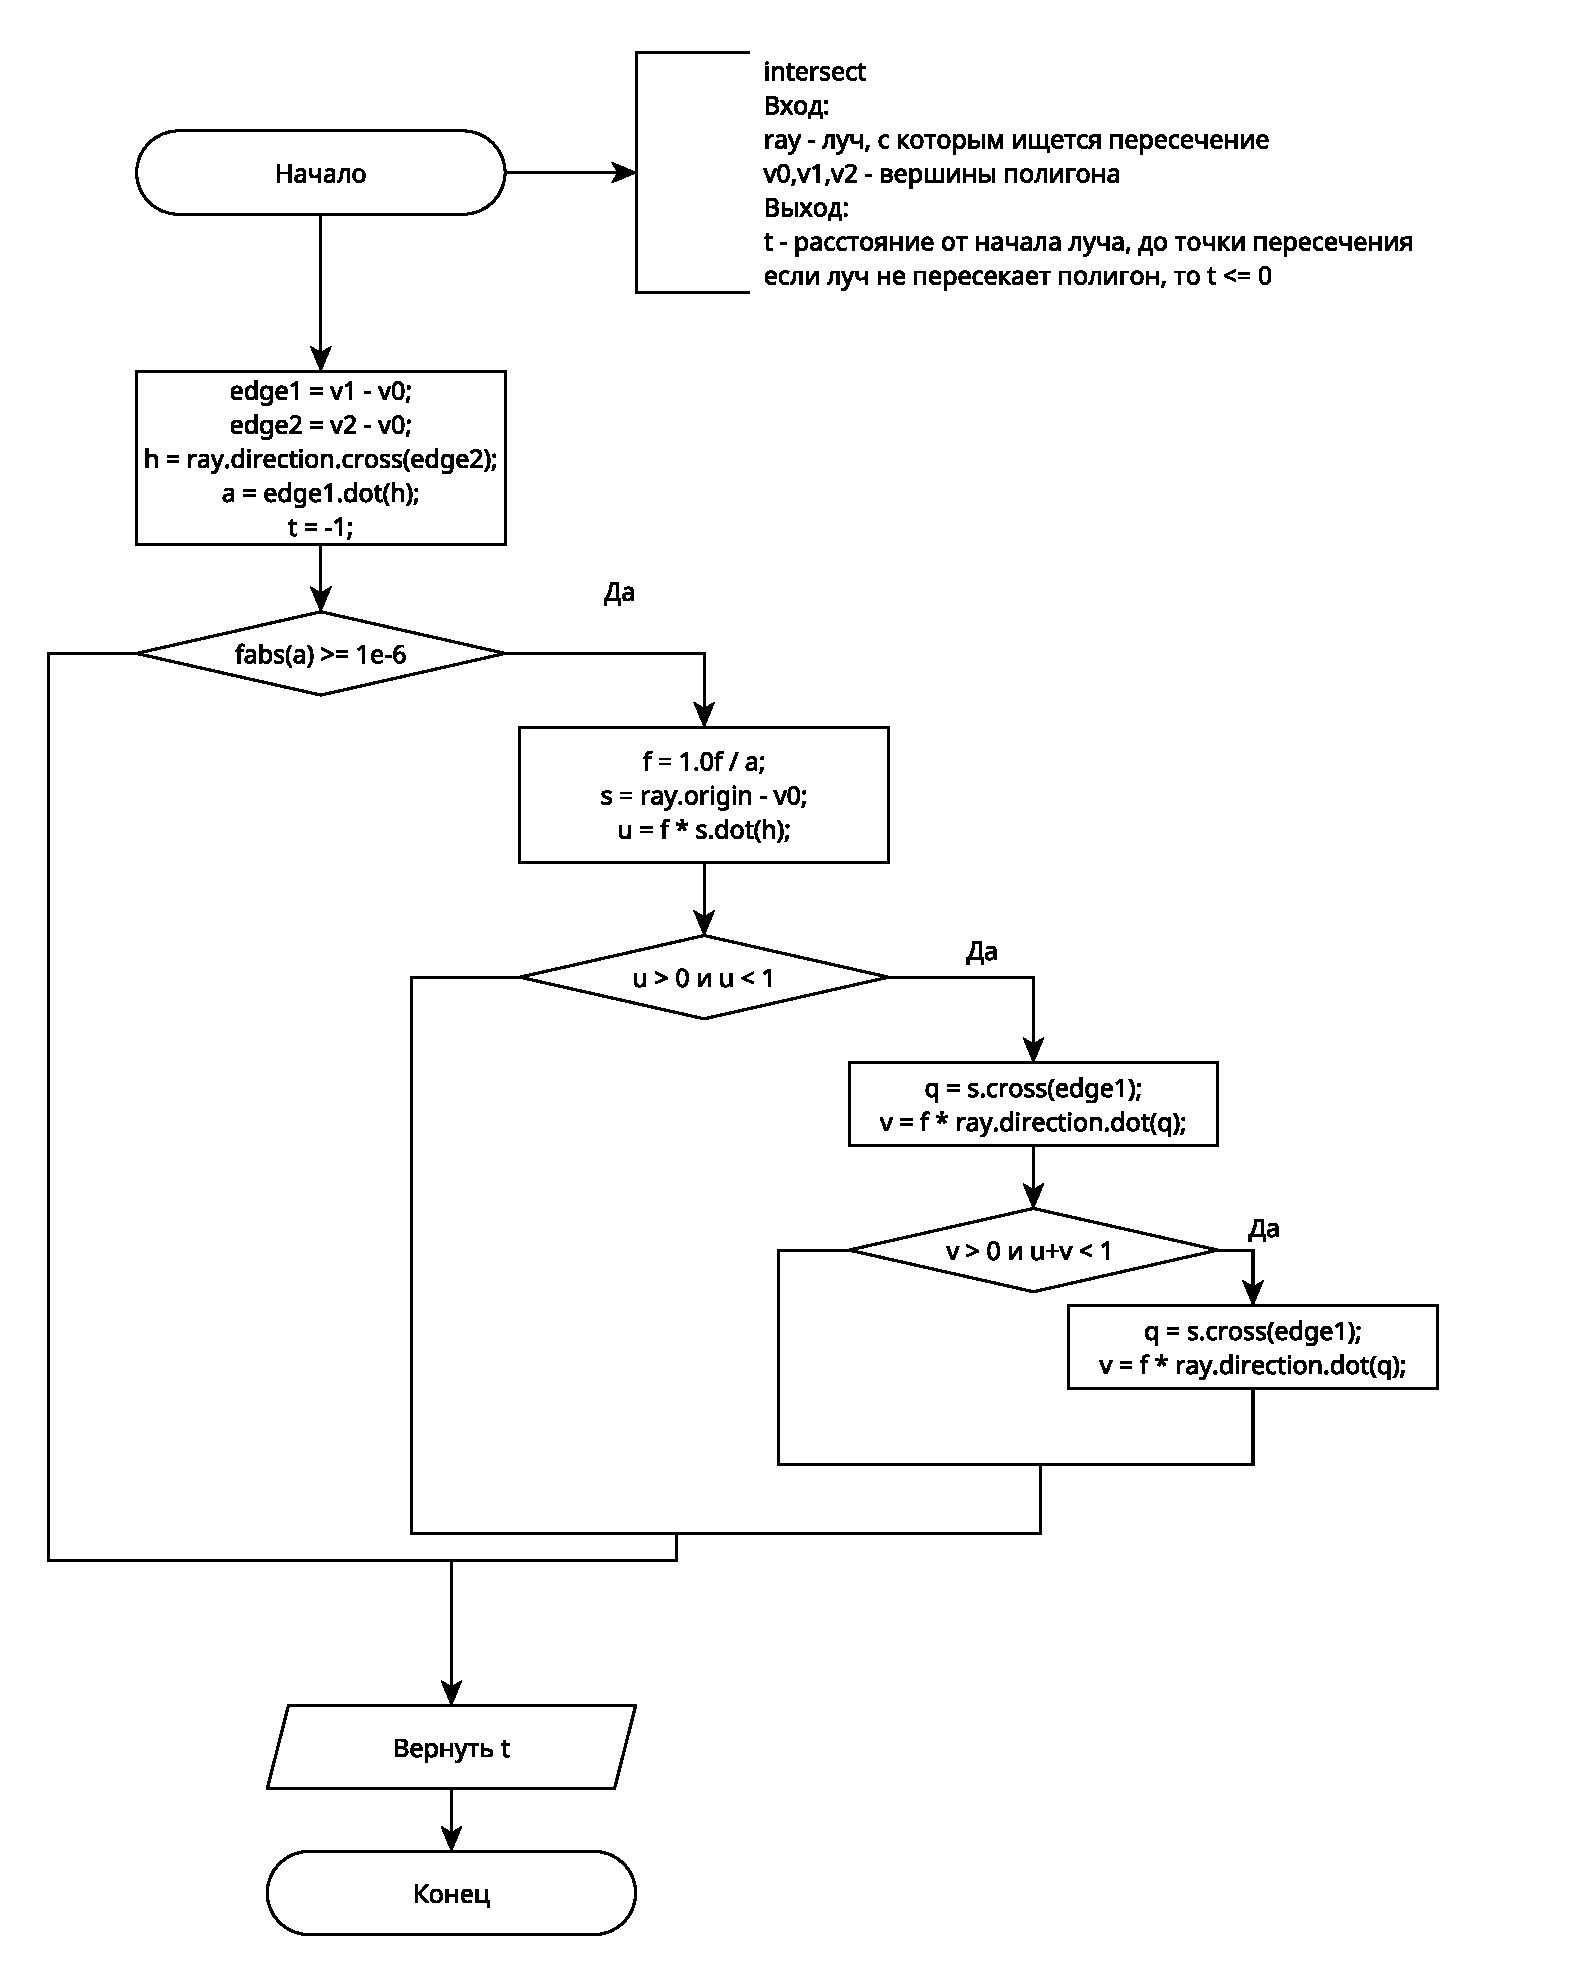
\includegraphics[width=\textwidth, height=210mm, width=170mm, keepaspectratio]{img/polygon_intersect.eps}}
		\caption{Схема алгоритма поиска пересечения с полигоном}
		\label{img/polygon_intersect}
	\end{figure}

\subsection{Персечение с оптической линзой}
Поскольку линза задается пересечением двух сфер, поиск персечения луча с ней сводится к поиск пересечения с этими сферами. Схема алгоритма представлена на рисунке \ref{img/lens_intersect}.
	\begin{figure}[H]
		\center{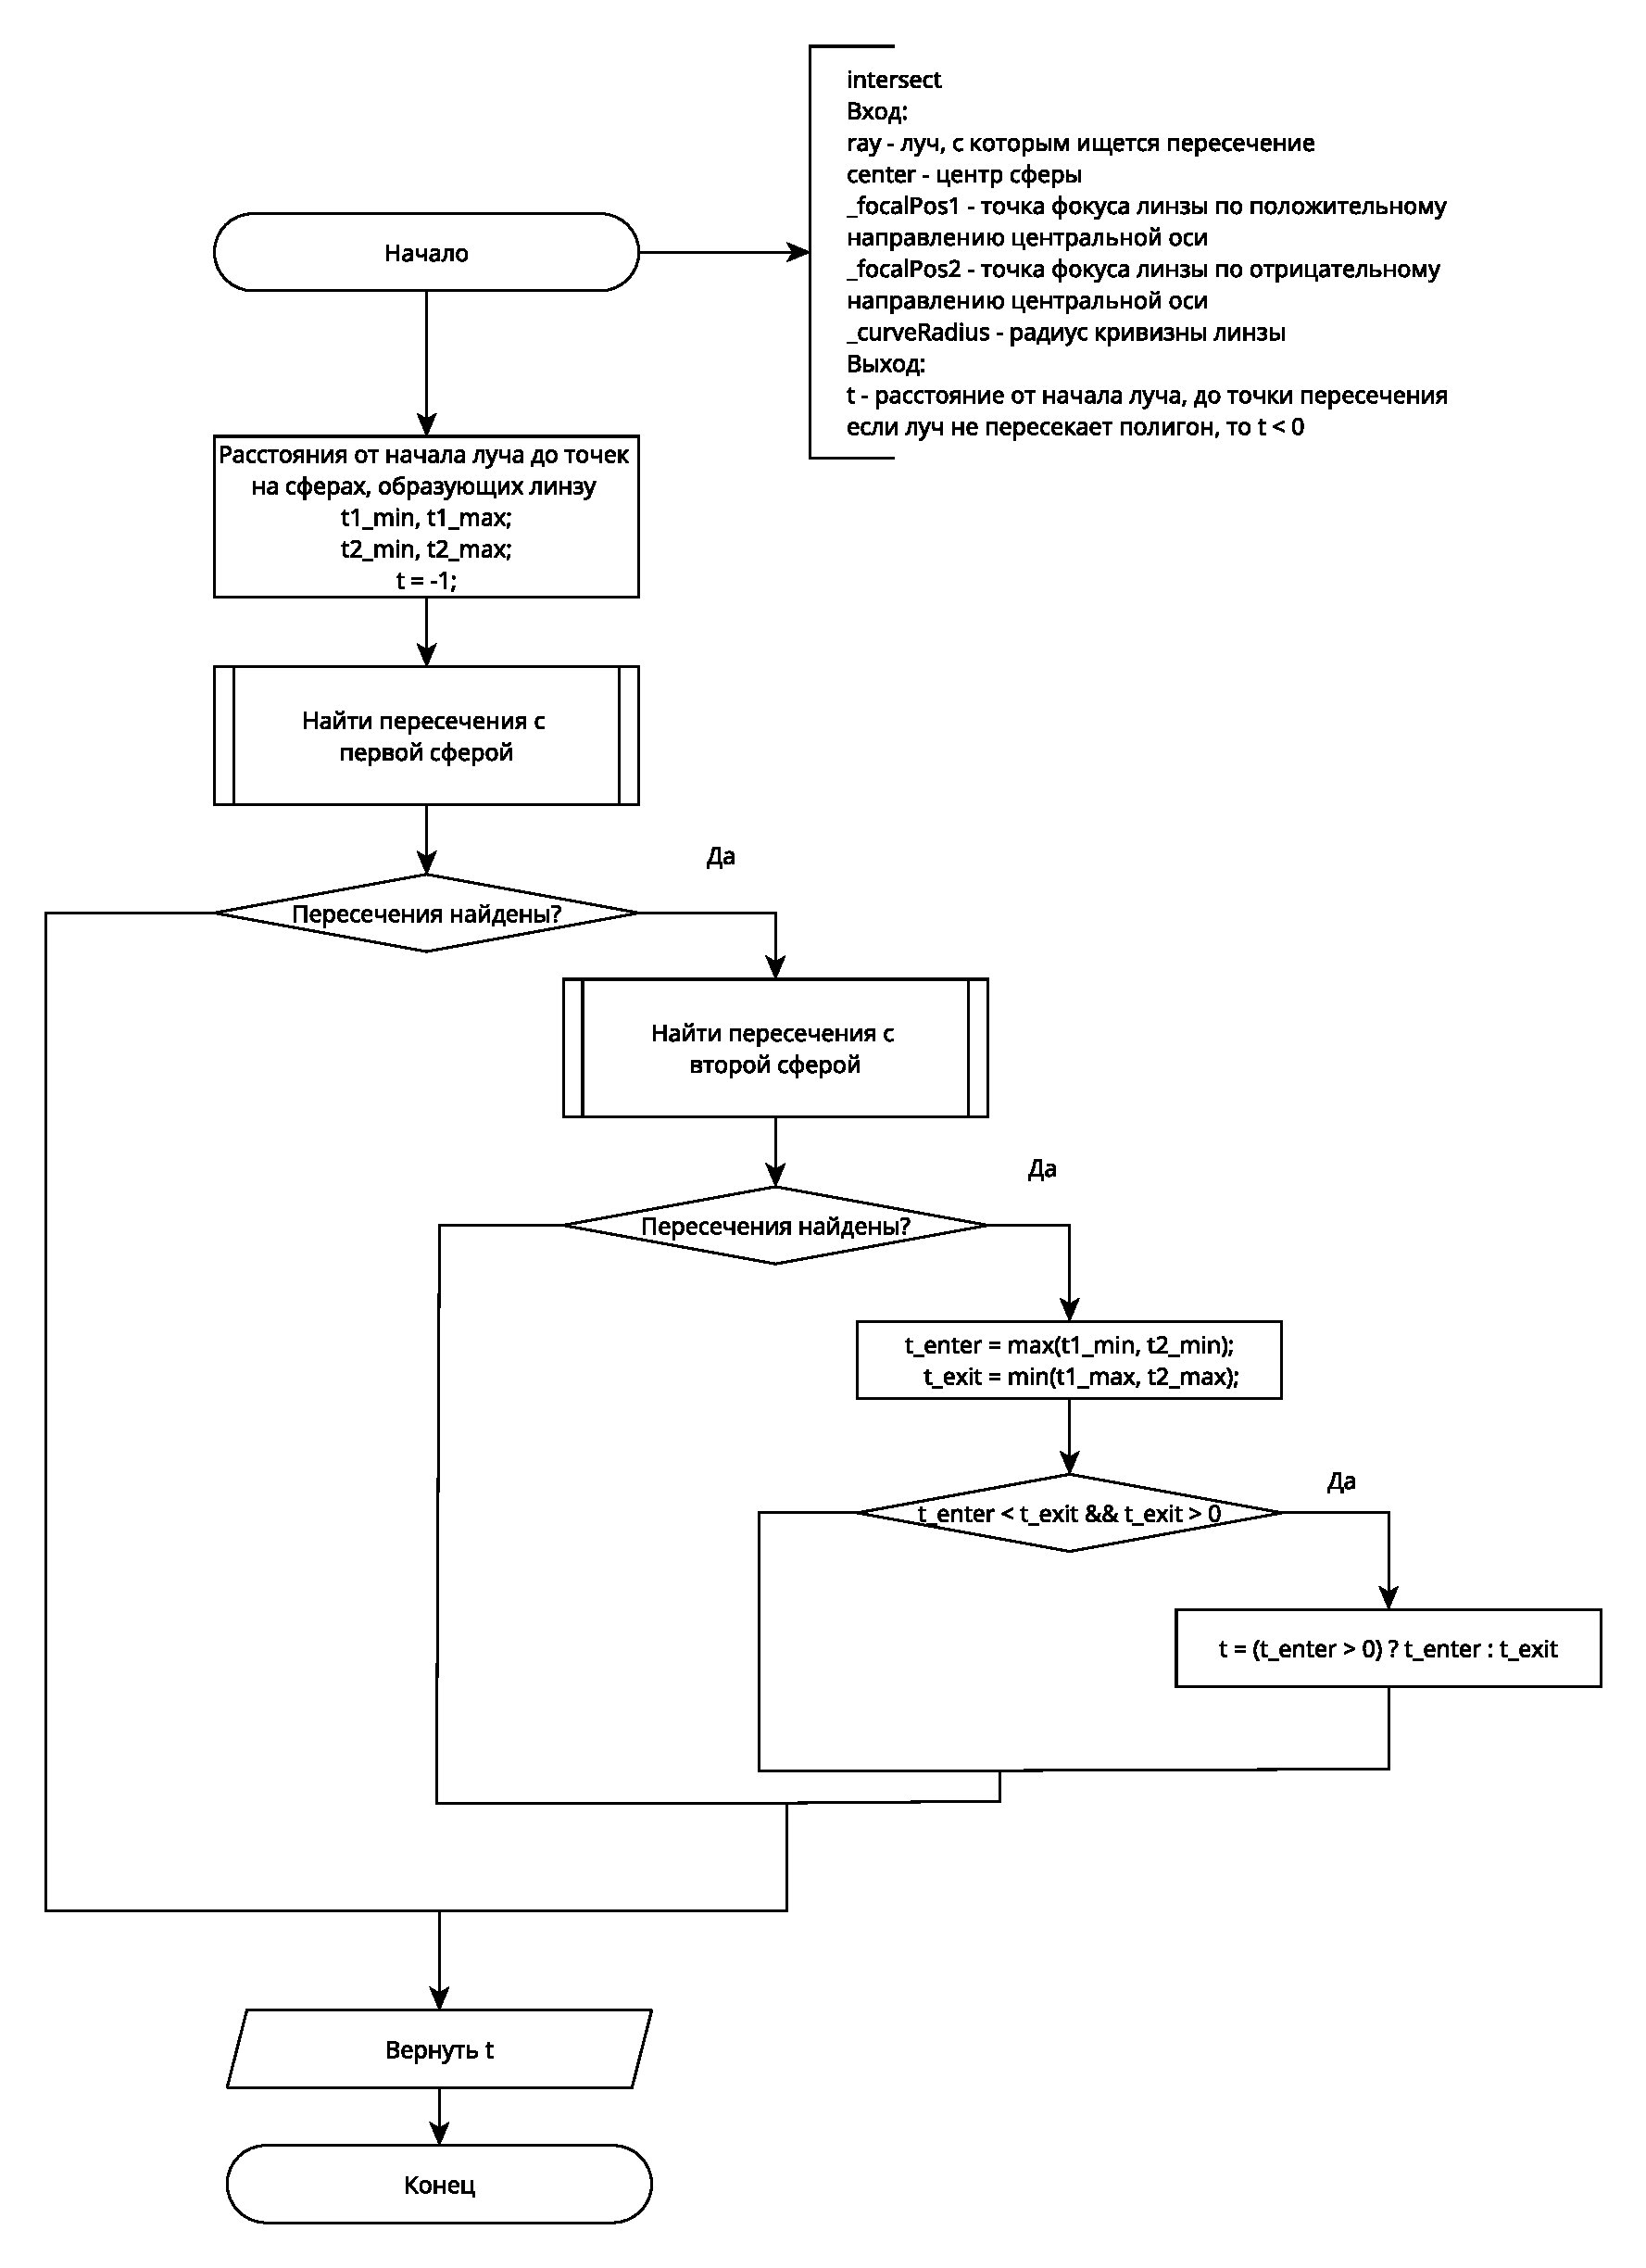
\includegraphics[width=\textwidth, height=210mm, width=170mm, keepaspectratio]{img/lens_intersect.eps}}
		\caption{Схема алгоритма поиска пересечения с линзой}
		\label{img/lens_intersect}
	\end{figure}
	
	\subsection{Обратная трассировка}
	Алгоритм заключается в трассировке лучей от наблюдателя, пока не превысится глубина рекурсивного поиска или луч не будет пересекаться ни с одним объектом сйены. При пересечении с объектом испускается отраженный и преломленный если соответвенно коэффициенты отражения и прозрачности объекта больше 0. Схема алгоритма представлена на рисунках \ref{img/raytracer_1} - \ref{img/raytracer_2}.
	\begin{figure}[H]
		\center{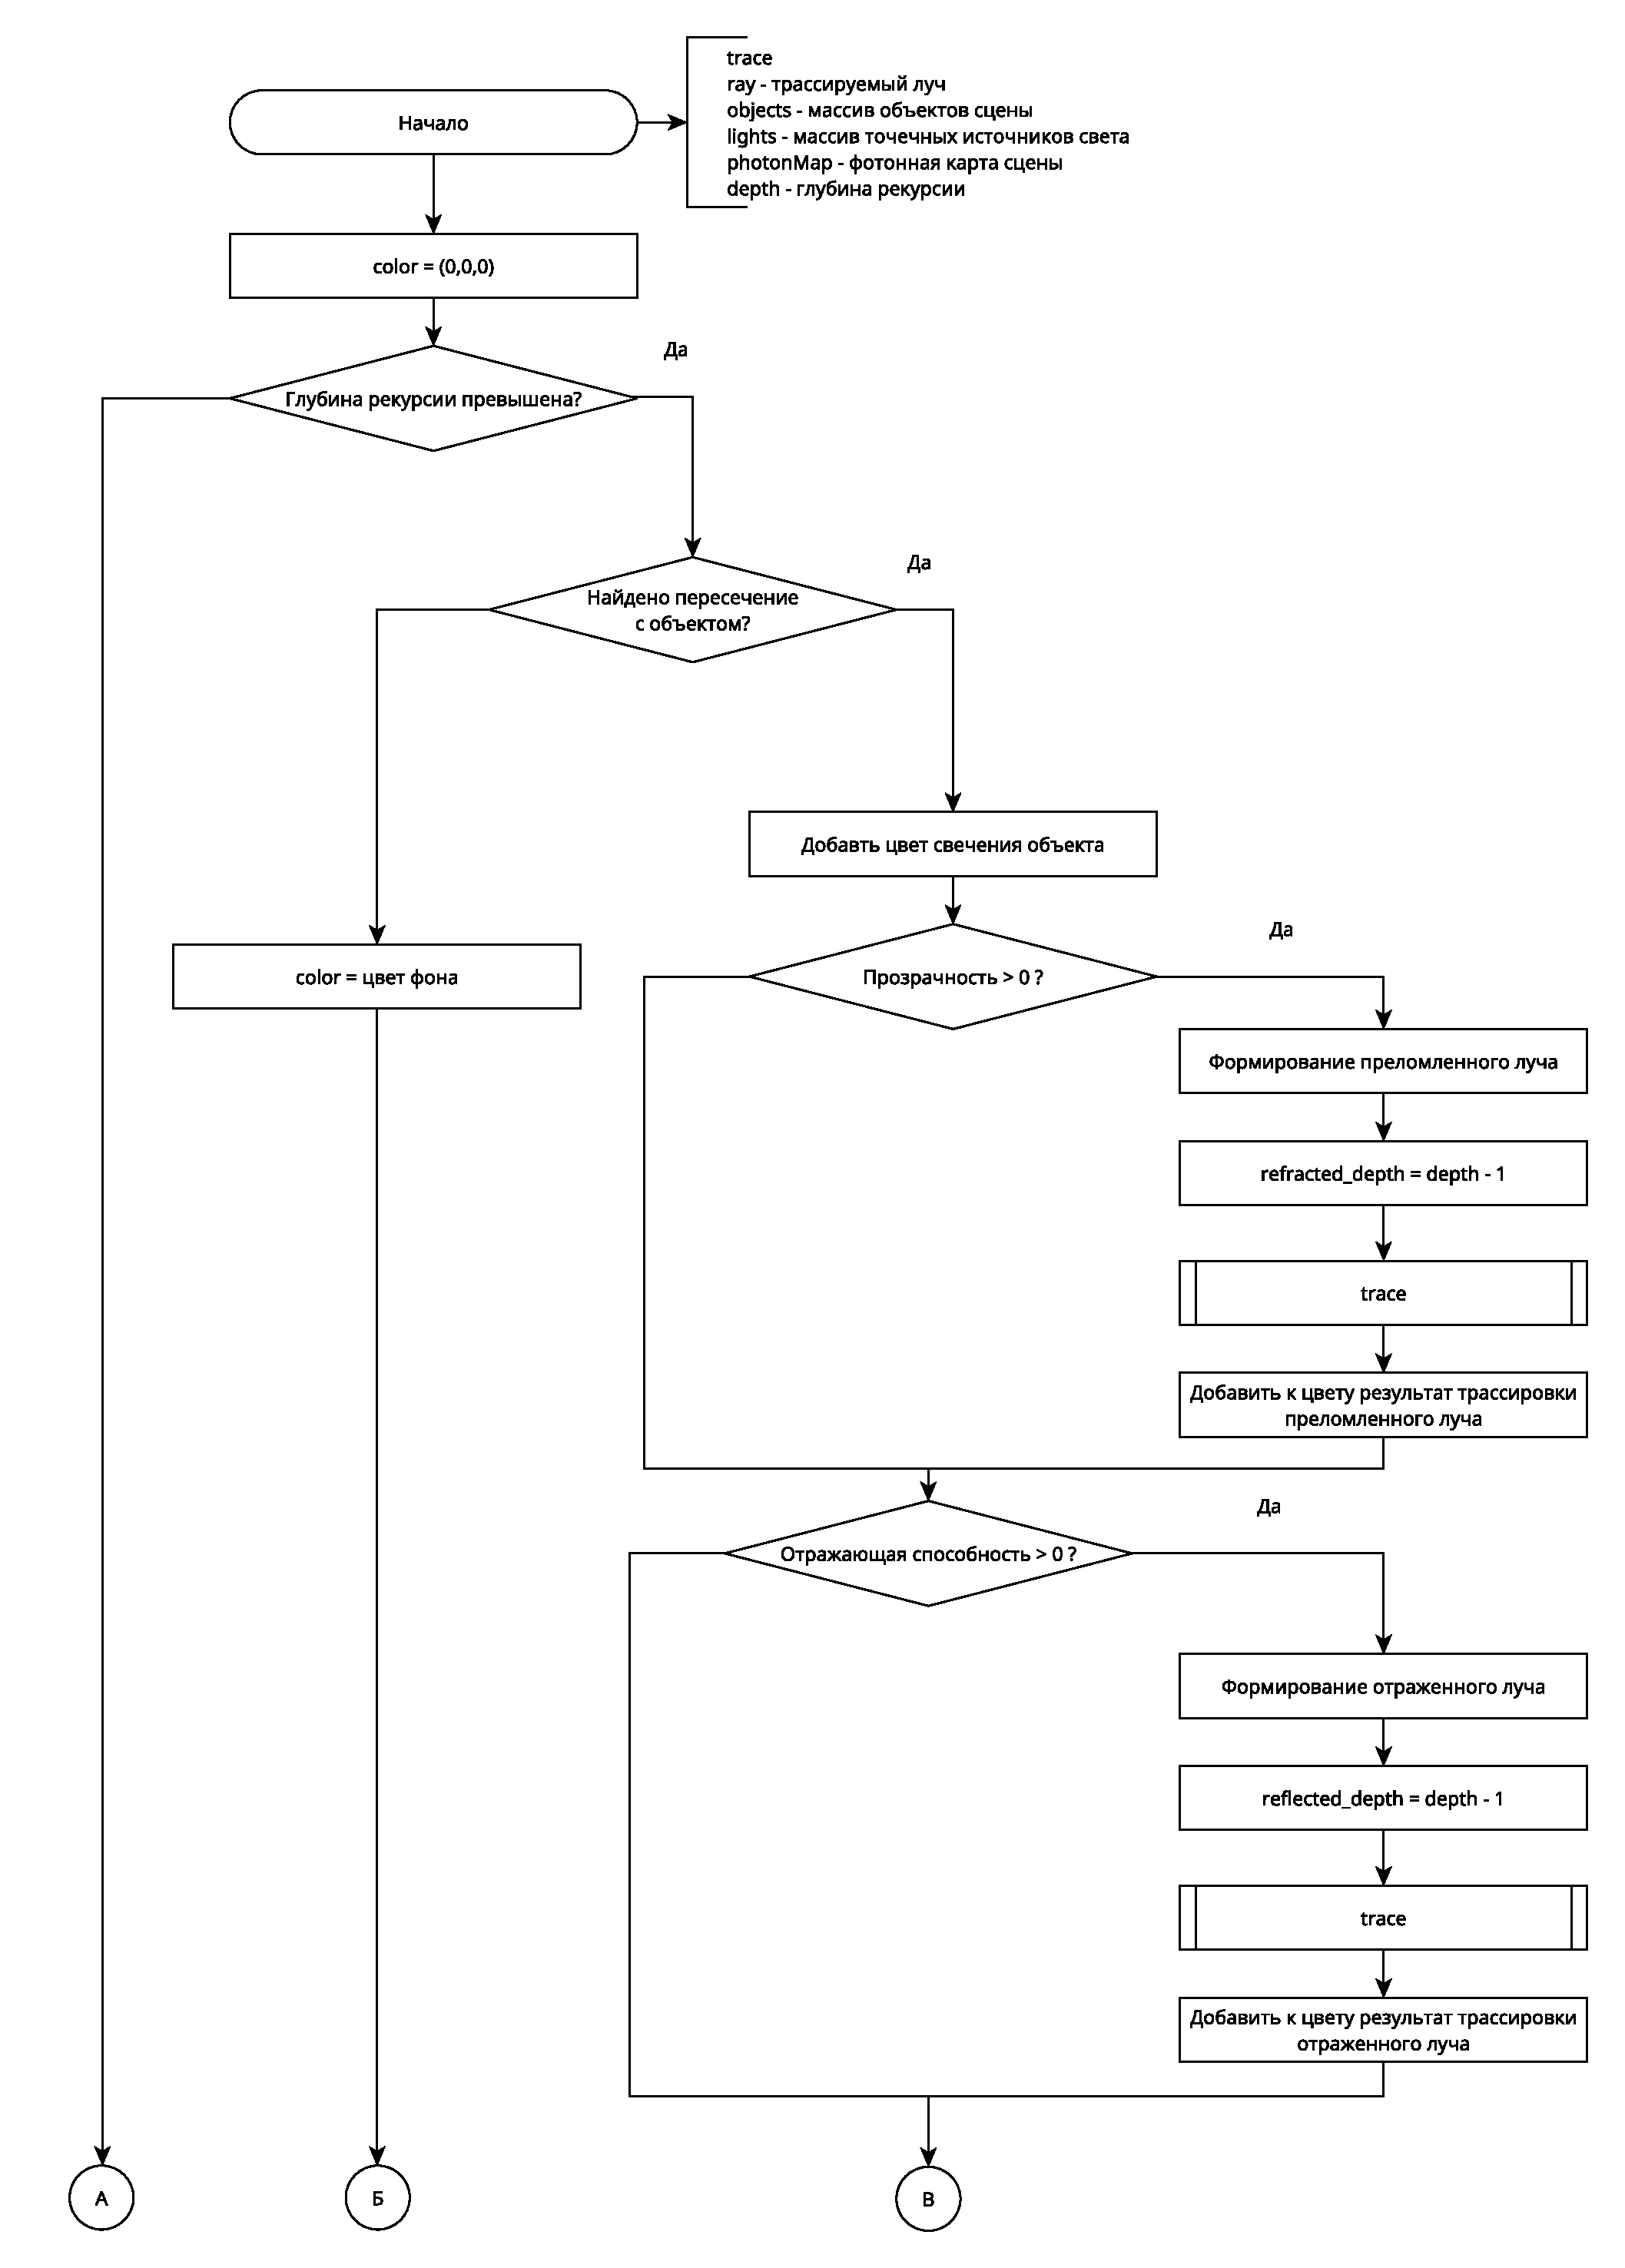
\includegraphics[width=\textwidth, height=210mm, width=170mm, keepaspectratio]{img/raytracer_1.eps}}
		\caption{Схема алгоритма обратной трассировки (часть 1)}
		\label{img/raytracer_1}
	\end{figure}
	
	\begin{figure}[H]
		\center{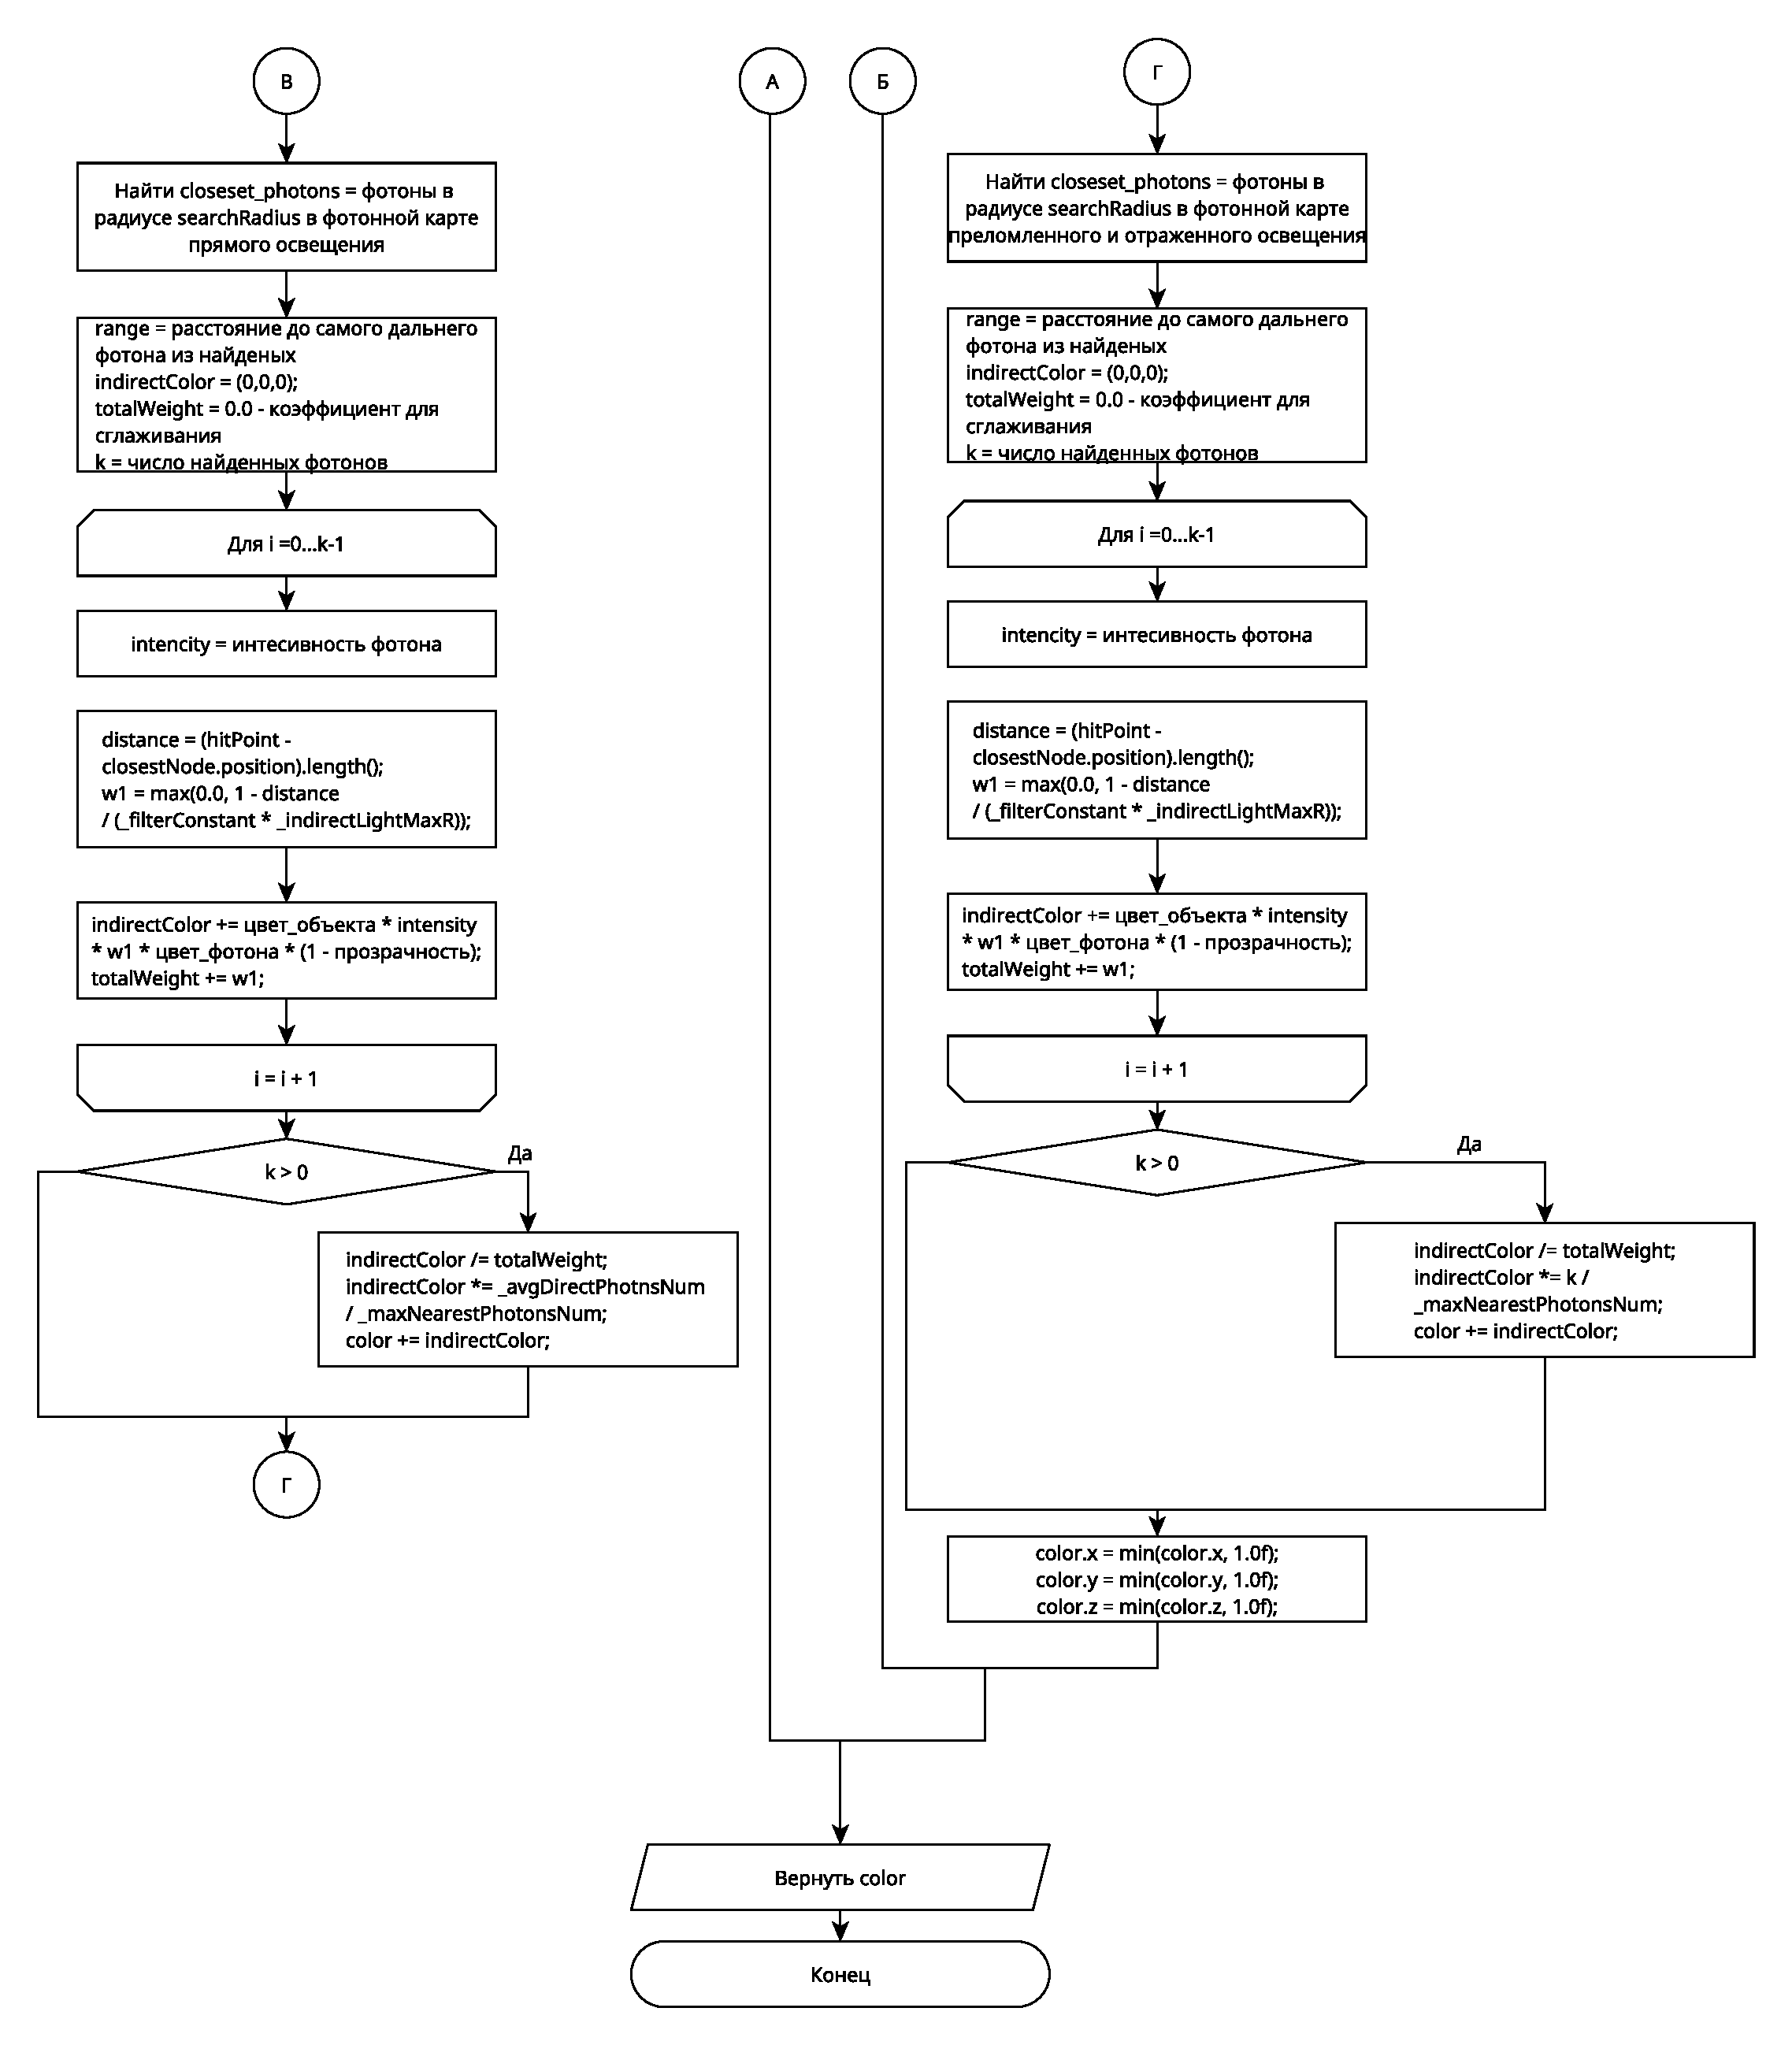
\includegraphics[width=\textwidth, height=210mm, width=170mm, keepaspectratio]{img/raytracer_2.eps}}
		\caption{Схема алгоритма обратной трассировки (часть 2)}
		\label{img/raytracer_2}
	\end{figure}
	
\subsection{Алгоритм построения фотонной карты}

Фотонная карта хранит пересечения фотонов с объектами ввиде K-мерного дерева. При построении карты по списку фотонов список сначала упорядочивается по оси $X$, разбивается пополам, и происходит рекурсивный вызов функции. На следующем шаге рекурсии разбиение происходит по оси $Y$, потом $Z$, посе чего снова по $X$. Схема алгоритма представлена на рисунке \ref{img/photonmap}.
 
	\begin{figure}[H]
		\center{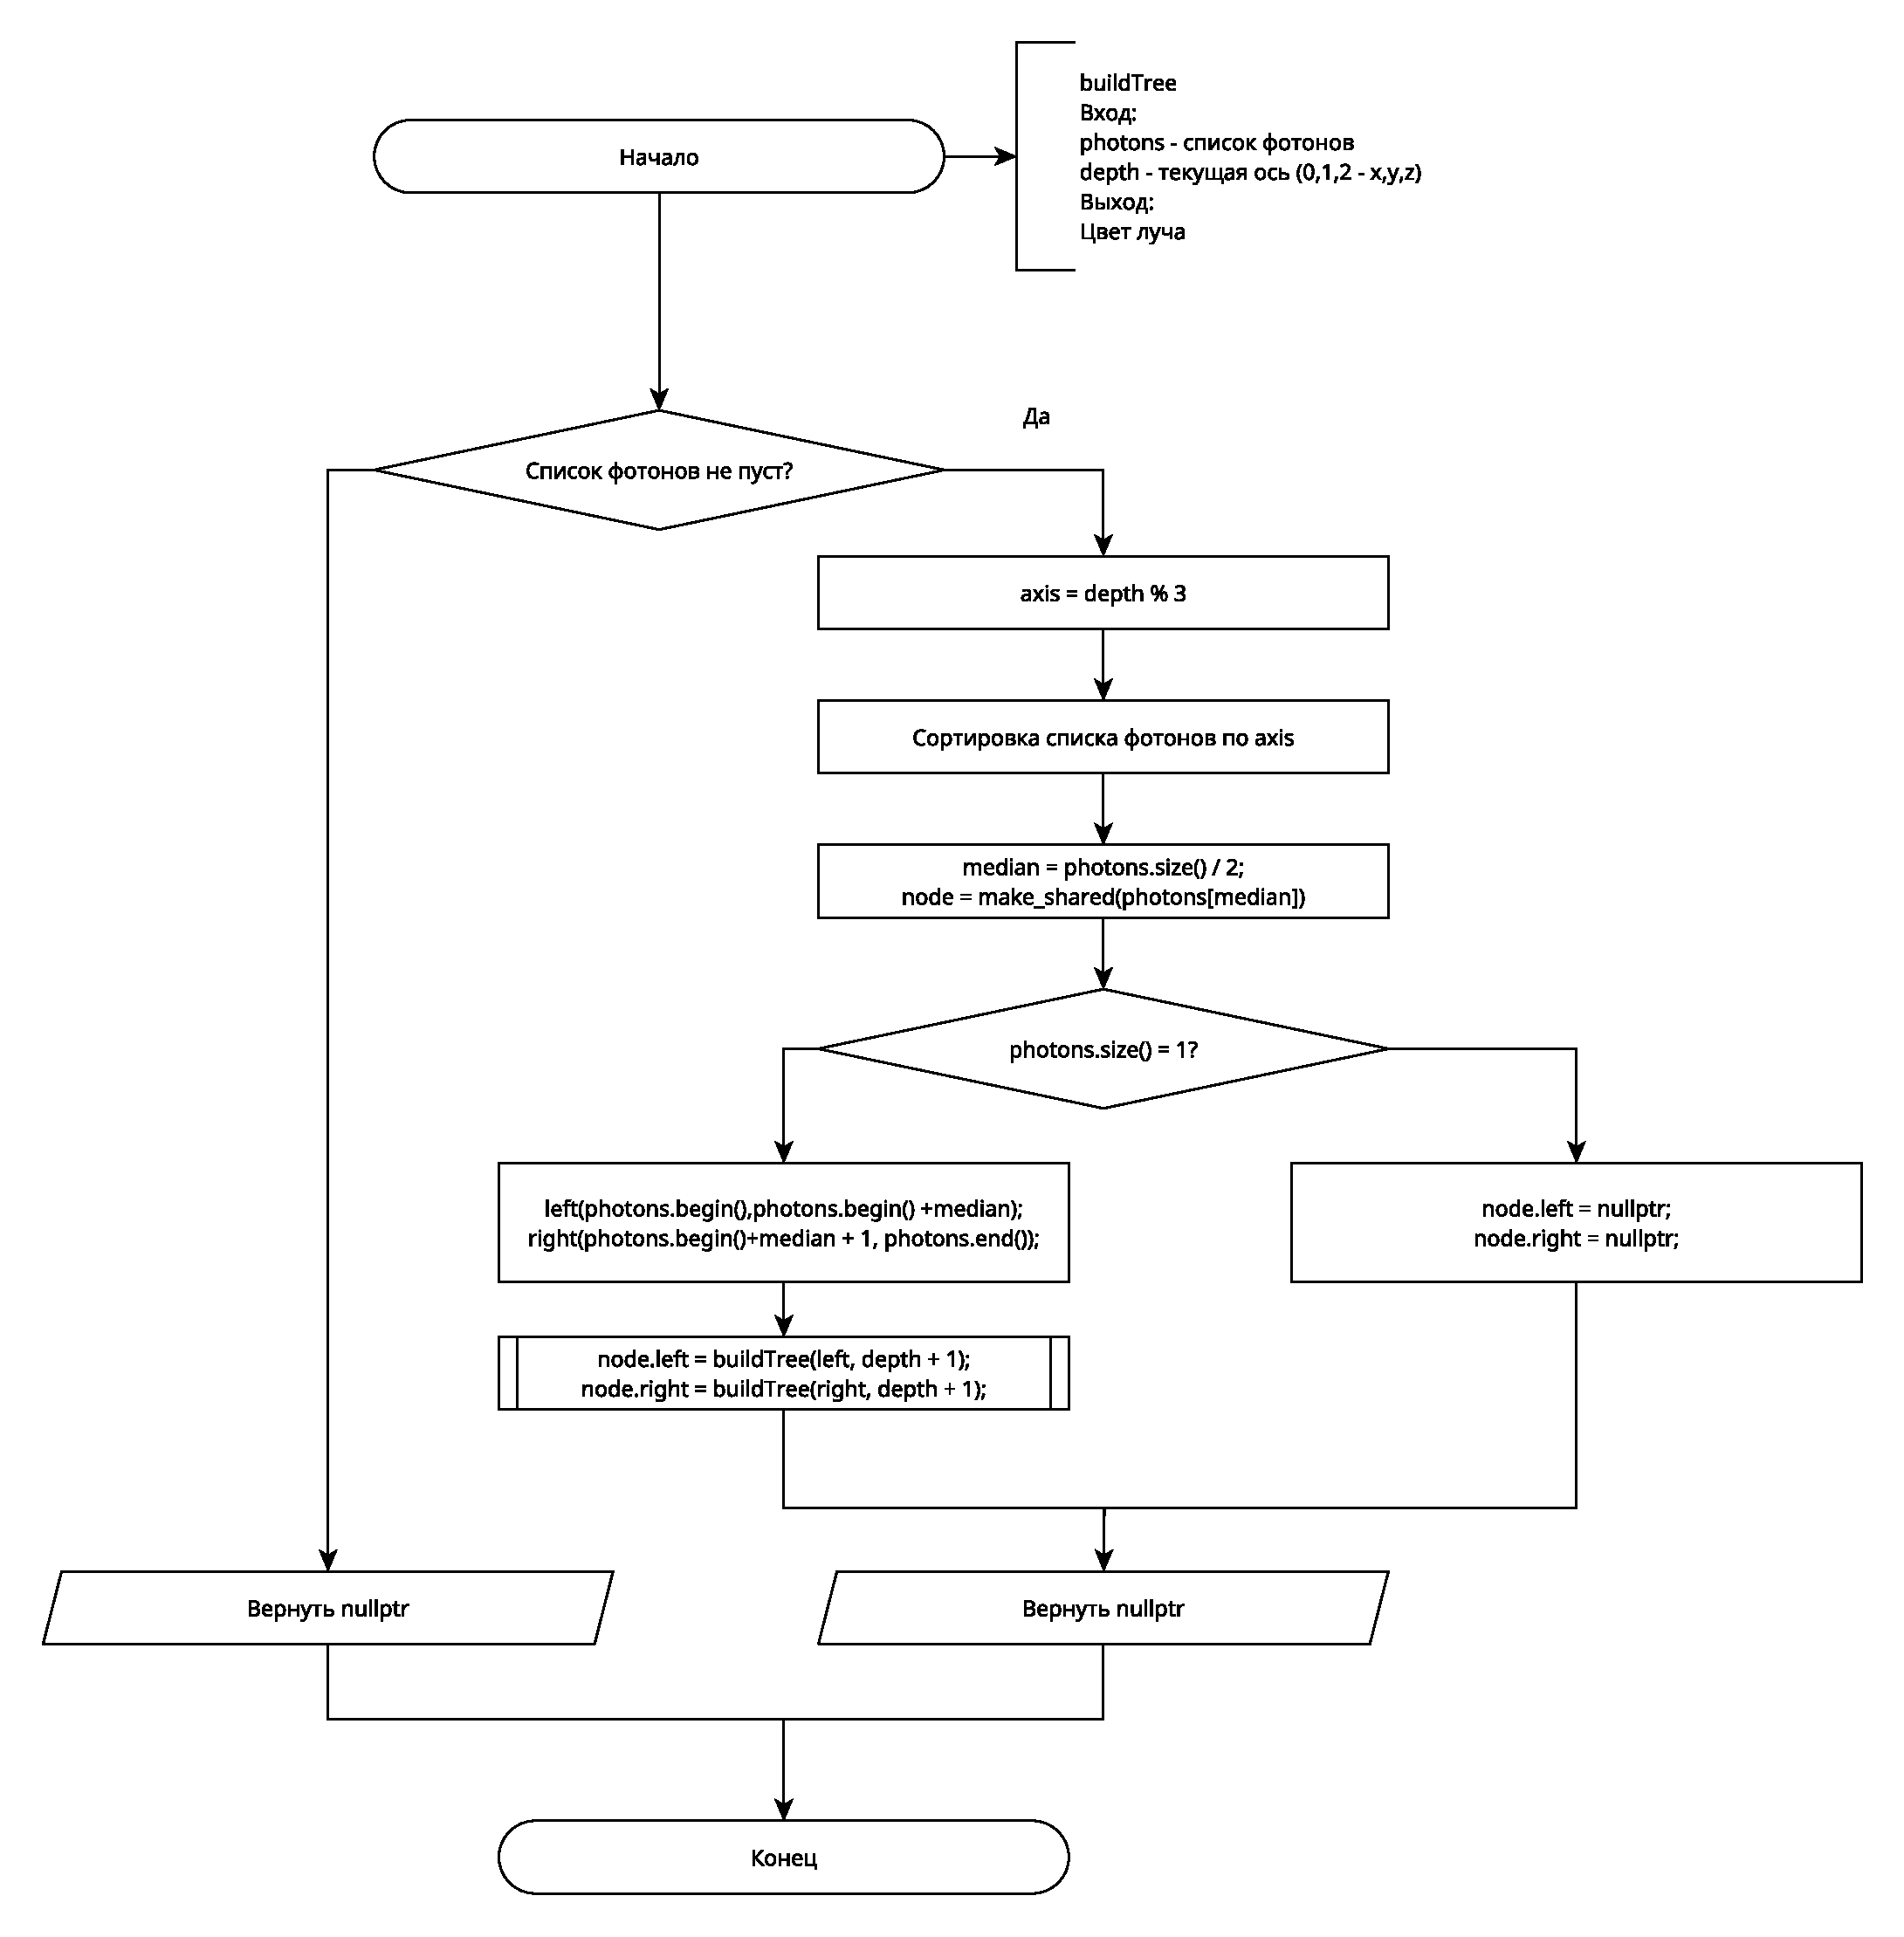
\includegraphics[width=\textwidth, height=210mm, width=170mm, keepaspectratio]{img/photonmap.eps}}
		\caption{Схема алгоритма построения фотонной карты по списку фотонов}
		\label{img/photonmap}
	\end{figure}

	
	
\chapter{Технологическая часть}

    В разделе представлены средства разработки программного обеспечения и детали реализации.
    
    \section{Средства реализация}
	Для реализации программного обеспечения выбран язык С++ \cite{cpp}. Выбор обуславливается тем, что язык представляет весь необходимый для решения поставленной задачи функционал.      

        Для создания пользовательского интерфейса ПО был использован фреймворк QT\cite{qt}. Фреймворк содержит объекты, позволяющие напрямую работать с пикселями изображения, а  так же возможности создания интерактивных пользовательских интерфейсов.
        
        Для сборки программного обеспечения использовался инструмент QMake\cite{qt}.
        
        В качестве среды разработки была выбрана среда разработки QtCreator\cite{qt}.

\section{Используемые классы}

Используемые классы представлены на рисунке \ref{img/uml1}. Класс BaseObject является базовым для объектов сцены, класс Camera содержит описание наблюдателя, класс Scene хранит объекты сцены, наблюдателя и фотонные карты прямого и непрямого освещения сцены. В классе Вrawer реализованы функции, отвечающие за построения изображения сцены.

\begin{figure}[H]
		\center{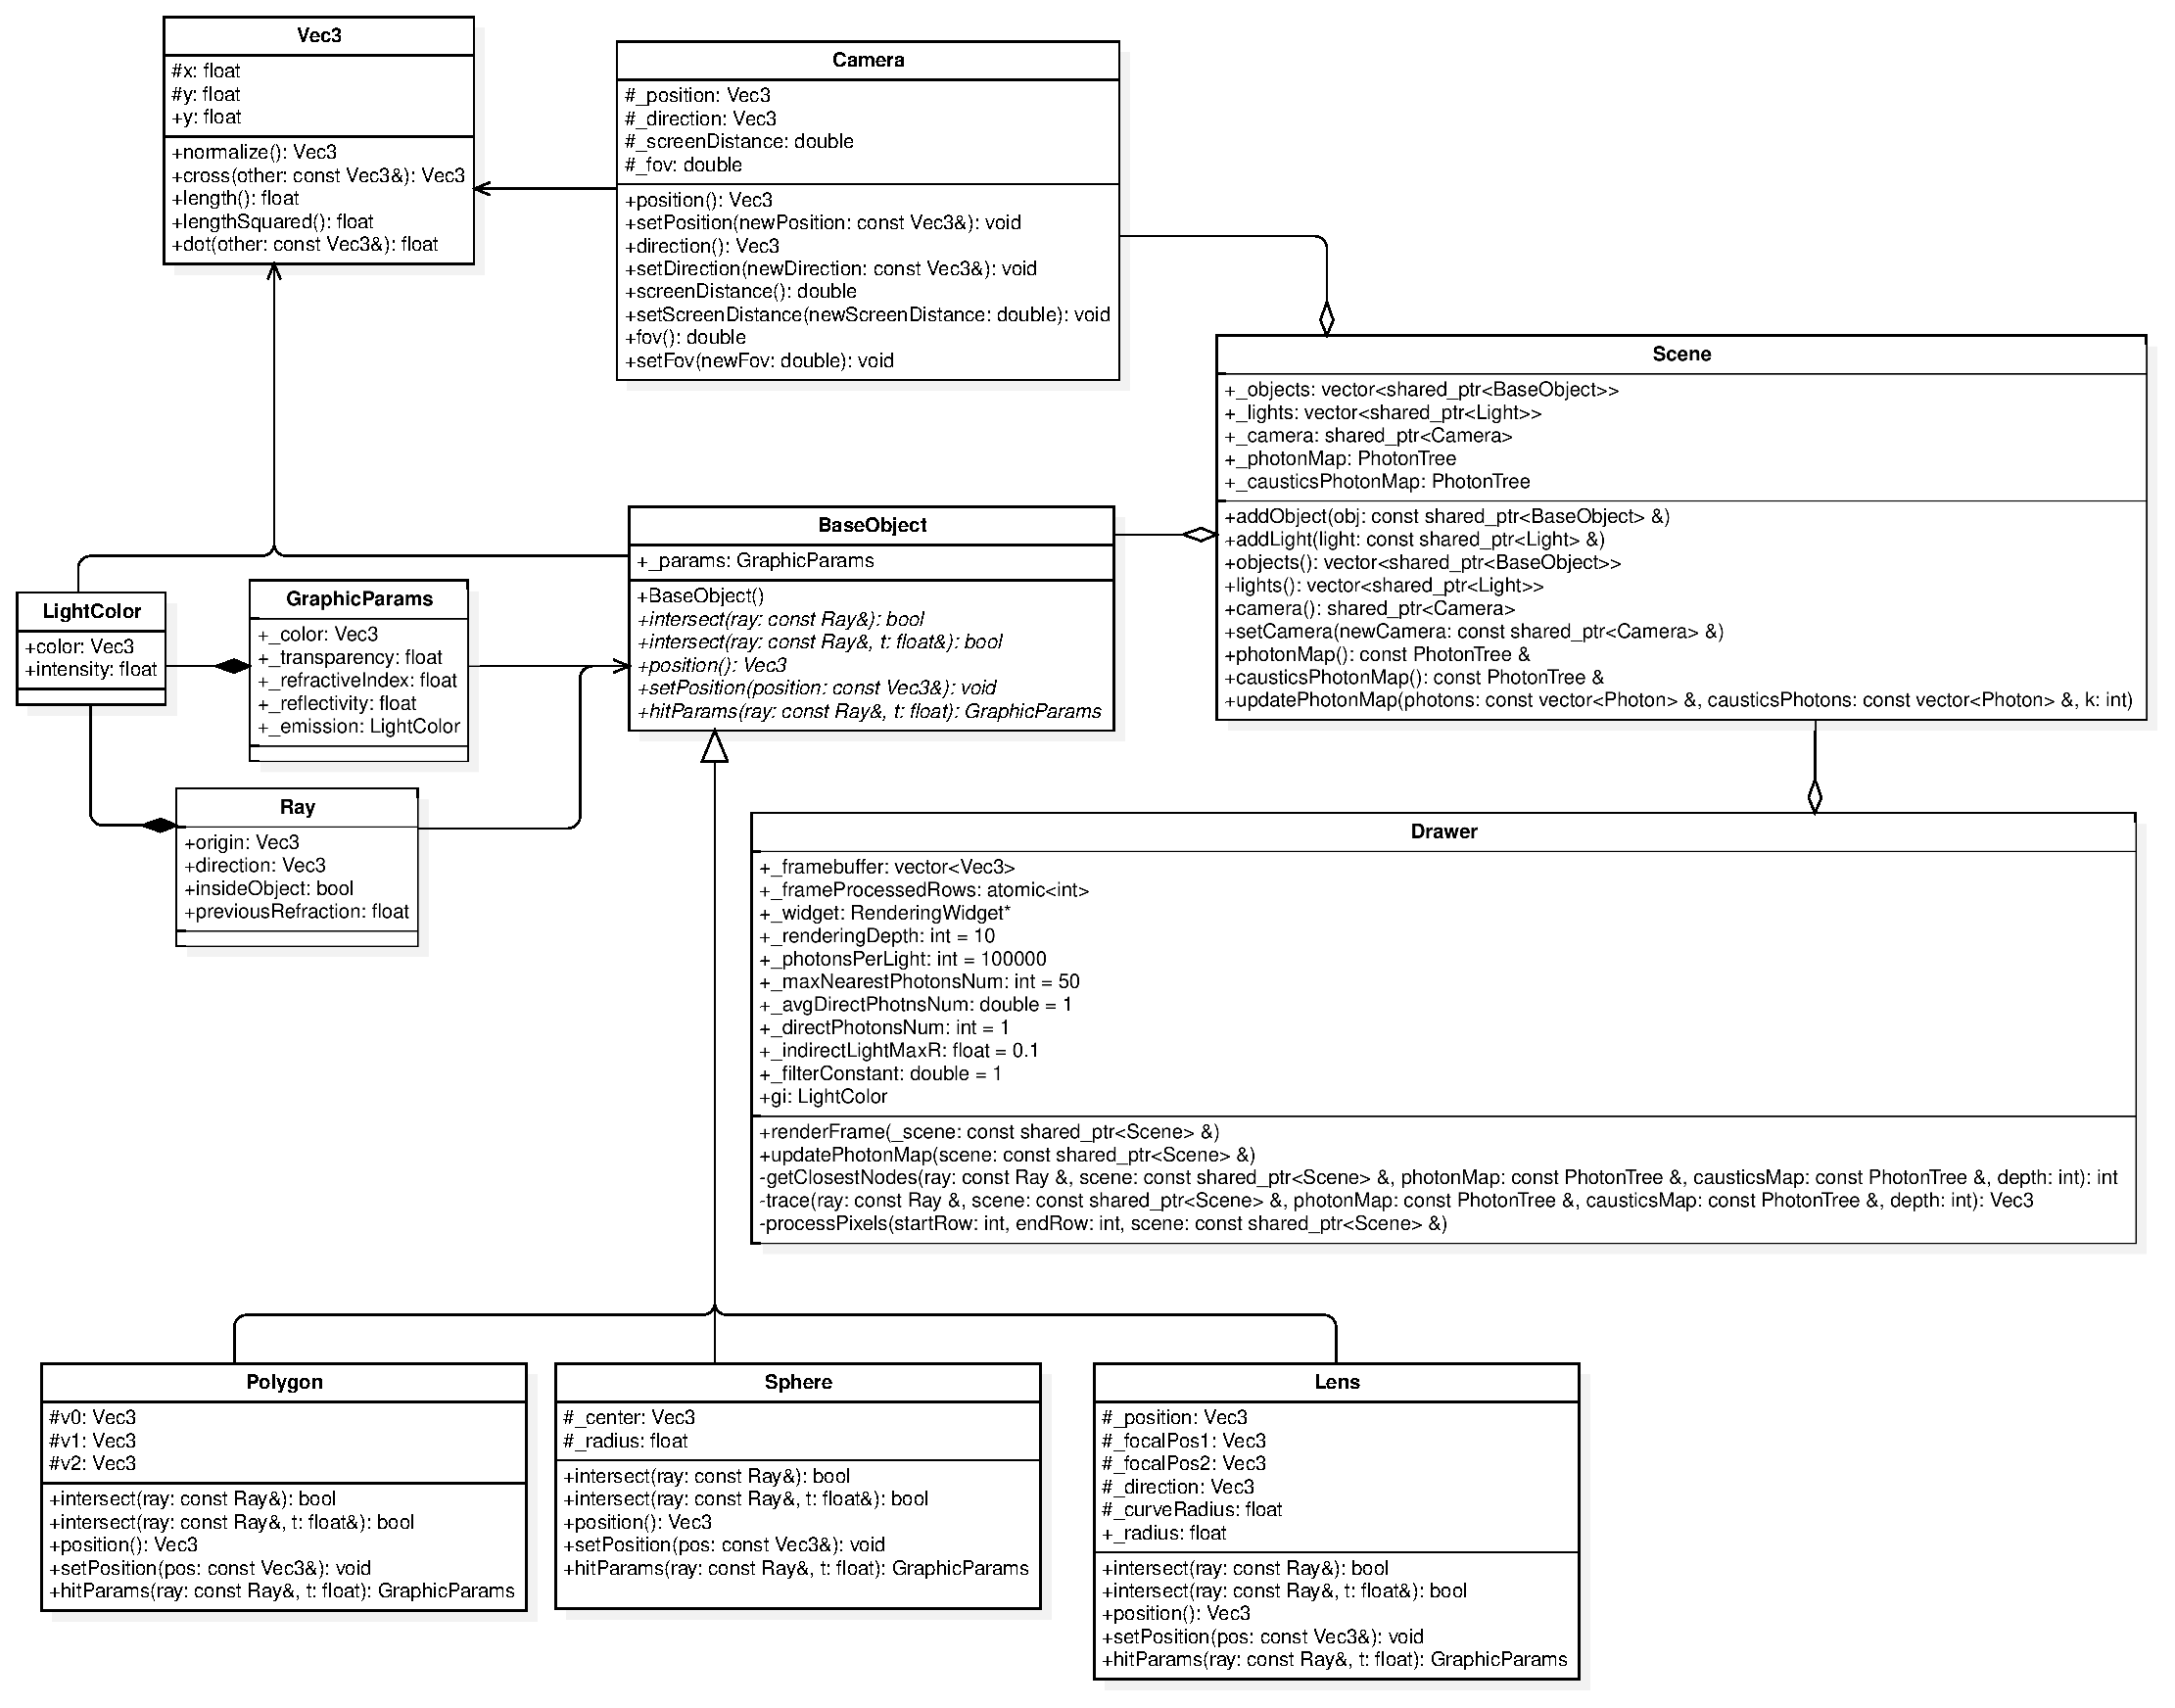
\includegraphics[width=\textwidth, height=210mm, width=170mm, keepaspectratio]{img/uml_1.eps}}
		\caption{UML диаграмма используемых классов}
		\label{img/uml1}
\end{figure}

    \section{Пользовательский интерфейс}
    
        Интерфейс реализуемого ПО представлен на рисунках \ref{img/ui_render} – \ref{img/ui}.
        

На рисунке \ref{img/ui_render} представлены параметры отрисовки, пользователь может задать число фотонов, испускаемых каждым источником света, радиус сбора освещенности и коснтанту фильтра, который используется в алгоритме сбора освещенности от ближайших фотонов, определяя влияния расстояния от точки до фотона на освещенность от этого фотона.
\begin{figure}[H]
		\center{\includegraphics[width=\textwidth, height=210mm, width=170mm, keepaspectratio]{img/ui_render.png}}
		\caption{Виджет параметров отрисовки}
		\label{img/ui_render}
\end{figure}
     
    На рисунке \ref{img/ui_camera} представлены параметры наблюдателя. Пользователь может задать положения камеры, направление ее взгляда и угол обзора.
\begin{figure}[H]
		\center{\includegraphics[width=\textwidth, height=210mm, width=170mm, keepaspectratio]{img/ui_camera.png}}
		\caption{Виджет параметров камеры}
		\label{img/ui_camera}
\end{figure}

На рисунке \ref{img/ui_sphere} представлены параметры сферы на сцене. Пользователь может определить положение, радиус, прозрачность, зеркальность, коэффициент преломления, цвет поверхности сферы, цвет и интенсивность излучения сферы.
\begin{figure}[H]
		\center{\includegraphics[width=\textwidth, height=210mm, width=170mm, keepaspectratio]{img/ui_sphere.png}}
		\caption{Виджет параметров сферы}
		\label{img/ui_sphere}
\end{figure}

На рисунке \ref{img/ui_polygon} представлены параметры треугольного полигона. Есть возможность задать положение трех его точек и графические параметры.
\begin{figure}[H]
		\center{\includegraphics[width=\textwidth, height=210mm, width=170mm, keepaspectratio]{img/ui_polygon.png}}
		\caption{Виджет параметров полигона}
		\label{img/ui_polygon}
\end{figure}

На рисунке \ref{img/ui_lens} представлены параметры линзы, имеется возможность изменить радиус кривизны, общий радиус, графические параметры и положение в пространстве.
\begin{figure}[H]
		\center{\includegraphics[width=\textwidth, height=210mm, width=170mm, keepaspectratio]{img/ui_lens.png}}
		\caption{Виджет параметров линзы}
		\label{img/ui_lens}
\end{figure}
        
На рисунке \ref{img/ui} представлен пример работы программы с несколькими прозрачными объектами.
\begin{figure}[H]
		\center{\includegraphics[width=\textwidth, height=210mm, width=170mm, keepaspectratio]{img/ui.png}}
		\caption{Пример работы программы}
		\label{img/ui}
\end{figure}
    
    \section{Вывод}

        В разделе были представлены средства разработки программного обеспечения, детали реализации, пользовательский интерфейс. Также были проедемонстрированы примеры работы программы.
\chapter{Исследовательская часть}

    В данном разделе описан эксперимент по определению влияния числа фотонов, испускаемых источником света, и радиуса сбора освещенности на качество изображения и время его создания.
    
    \section{Цель эксперимента}
    
        Целью эксперимента является определение оптимального числа фотонов для отрисовки заданной сцены.
    
    \section{Технические характеристики}

        Технические характеристики устройства, на котором выполнялось исследование:

        \begin{itemize}
        	\item[--] процессор: Intel Core™ i5-13420H \cite{i5} 2.1ГГц;
        	\item[--] память: 16 Гб;
        	\item[--] операционная система: Ubuntu 24.04.1 LTS \cite{ubuntu} Linux \cite{linux}.
        \end{itemize}
        
        Эксперимент проводился на ноутбуке, включенном в сеть электропитания, система работала в производительном режиме без ограничений на нагрузку процессора. Во время тестирования ноутбук был нагружен только встроенными приложениями окружения рабочего стола, окружением рабочего стола и непосредственно системой тестирования.
        
    \section{Описание эксперимента}

        Создана сцена состоящая из 2 прозрачных, 1 непрозрачного объекта и источника света. По сцене строилось изображение размером 900x900 пикселей для разного числа фотонов, испускаемых источником: от 100000 до 1100000 с шагом в 250000 фотонов, радиус сбора освещенности: от 0.05 до 0.1 с шагом 0.25. Рассматриваемя сцена представлена на рисунке \ref{img/full_experiment}.

        \begin{figure}[H]
		\center{\includegraphics[width=\textwidth, height=210mm, width=170mm, keepaspectratio]{img/measures/full.png}}
		\caption{Сцена эксперимента}
		\label{img/full_experiment}
\end{figure}
 
        
\section{Зависимость времени построения карты от числа фотонов на источник}

В таблице \ref{tbl:render_time} представлена зависимость времени построения карты от числа фотонов на источник. Исследование проводилось при различных значениях числа фотонов.

\begin{table}[h]
    \centering
    \small
    \caption{Время построения карты в зависимости от числа фотонов}
    \label{tbl:render_time}
    \begin{tabular}{
          |>{\raggedleft\arraybackslash}m{1.7in}|
          >{\raggedleft\arraybackslash}m{1.7in}|}
        \hline
        Число фотонов на источник & Время построения (c) \\
        \hline
        100000   & 1.794 \\
        \hline
        350000   & 6.722 \\
        \hline
        600000   & 11.948 \\
        \hline
        850000   & 17.718 \\
        \hline
        1100000  & 23.214 \\
        \hline
    \end{tabular}
\end{table}

По таблице \ref{tbl:render_time} построен график, изображенный на рисунке \ref{img:render_graph}.

\begin{figure}[h]
    \begin{center}
        \begin{tikzpicture}
            \begin{axis}[
                title={Время построения карты},
                xlabel={Число фотонов на источник},
                ylabel={Время построения (c)},
                width=12cm,
                grid=major,
                smooth,
                legend pos=outer north east,
            ]
            \addplot coordinates {(100000, 1.794) (350000, 6.722) (600000, 11.948) (850000, 17.718) (1100000, 23.214)};
            \addlegendentry{Время построения}
            \end{axis}
        \end{tikzpicture}
    \end{center}
    \captionsetup{justification=centering}
    \caption{График зависимости времени построения карты от числа фотонов на источник}
    \label{img:render_graph}
\end{figure}

По результатам видно, что время построения карты линейно зависит от числа фотонов, испускаемых источником.

\clearpage

\section{Зависимость времени отрисовки от радиуса сбора освещенности}

В таблице \ref{tbl:collection_radius} представлена зависимость времени отрисовки от радиуса сбора освещенности. Исследование проводилось при различных радиусах и числах фотонов.

\begin{table}[h]
    \centering
    \small
    \caption{Зависимость времени отрисовки от радиуса сбора освещенности}
    \label{tbl:collection_radius}
    \begin{tabular}{
          |>{\raggedleft\arraybackslash}m{1.3in}|
          >{\raggedleft\arraybackslash}m{1.3in}|
          >{\raggedleft\arraybackslash}m{1.3in}|
          >{\raggedleft\arraybackslash}m{1.3in}|}
        \hline
        Радиус сбора & Число фотонов & Время (c) & Изображение \\
        \hline
        \multirow{5}{*}{0.025} & 100000 & 9.264 & Рисунок \ref{img/0025100} \\
        & 350000 & 16.019 & Рисунок \ref{img/0025350} \\
        & 600000 & 20.838 & Рисунок \ref{img/0025600} \\
        & 850000 & 25.42 & Рисунок \ref{img/0025850} \\
        & 1100000 & 29.201 & Рисунок \ref{img/00251100} \\
        \hline
        \multirow{5}{*}{0.050} & 100000 & 12.602 & Рисунок \ref{img/005100} \\
        & 350000 & 25.423 & Рисунок \ref{img/005350} \\
        & 600000 & 36.297 & Рисунок \ref{img/005600} \\
        & 850000 & 44.543 & Рисунок \ref{img/005850} \\
        & 1100000 & 55.177 & Рисунок \ref{img/0051100} \\
        \hline
        \multirow{5}{*}{0.075} & 100000 & 16.722 & Рисунок \ref{img/0075100} \\
        & 350000 & 37.342 & Рисунок \ref{img/0075350} \\
        & 600000 & 56.473 & Рисунок \ref{img/0075600} \\
        & 850000 & 73.379 & Рисунок \ref{img/0075850} \\
        & 1100000 & 89.379 & Рисунок \ref{img/00751100} \\
        \hline
        \multirow{5}{*}{0.100} & 100000 & 22.153 & Рисунок \ref{img/01100} \\
        & 350000 & 53.549 & Рисунок \ref{img/01350} \\
        & 600000 & 83.571 & Рисунок \ref{img/01600} \\
        & 850000 & 110.001 & Рисунок \ref{img/01850} \\
        & 1100000 & 135.275 & Рисунок \ref{img/011100} \\
        \hline
    \end{tabular}
\end{table}

По таблице \ref{tbl:collection_radius} был построен график, изображенный на рисунке \ref{img:collection_graph}. По результатам можно сделать вывод, что время создания изображения имеет линейную зависимость от числа фотонов, испускаемых источником. 

\begin{figure}[h]
    \begin{center}
        \begin{tikzpicture}
            \begin{axis}[
                title={Время отрисовки в зависимости от числа фотонов на источник},
                xlabel={Число фотонов на источник},
                ylabel={Время отрисовки (c)},
                width=12cm,
                grid=major,
                legend pos=outer north east,
            ]
            % Радиус 0.1
            \addplot coordinates {(100000, 22.153) (350000, 53.549) (600000, 83.571) (850000, 110.001) (1100000, 135.275)};
            \addlegendentry{Радиус 0.1}

            % Радиус 0.075
            \addplot coordinates {(100000, 16.722) (350000, 37.342) (600000, 56.473) (850000, 73.379) (1100000, 89.379)};
            \addlegendentry{Радиус 0.075}

            % Радиус 0.05
            \addplot coordinates {(100000, 12.602) (350000, 25.423) (600000, 36.297) (850000, 44.543) (1100000, 55.177)};
            \addlegendentry{Радиус 0.05}

            % Радиус 0.0025
            \addplot coordinates {(100000, 9.264) (350000, 16.019) (600000, 20.838) (850000, 25.42) (1100000, 29.201)};
            \addlegendentry{Радиус 0.025}
            \end{axis}
        \end{tikzpicture}
    \end{center}
    \captionsetup{justification=centering}
    \caption{График зависимости времени отрисовки от числа фотонов}
    \label{img:collection_graph}
\end{figure}


На рисунке \ref{fig/measurements} представлены части изображений с наиболее характерными деффектами для разного радиуса сбора освещенности и числа фотонов.

\begin{figure}[htbp]
    \centering

    % Радиус 0.025
    \textbf{Рисунки для радиуса 0.025} \\
    \begin{minipage}{0.9\textwidth}
        \begin{subfigure}{0.18\textwidth}
            \includegraphics[width=\textwidth]{img/measures/0025100.png}
            \caption{Число фотонов: 100000.}
            \label{img/0025100}
        \end{subfigure}
        \hfill
        \begin{subfigure}{0.18\textwidth}
            \includegraphics[width=\textwidth]{img/measures/0025350.png}
            \caption{Число фотонов: 350000.}
            \label{img/0025350}
        \end{subfigure}
        \hfill
        \begin{subfigure}{0.18\textwidth}
            \includegraphics[width=\textwidth]{img/measures/0025600.png}
            \caption{Число фотонов: 600000.}
            \label{img/0025600}
        \end{subfigure}
        \hfill
        \begin{subfigure}{0.18\textwidth}
            \includegraphics[width=\textwidth]{img/measures/0025850.png}
            \caption{Число фотонов: 850000.}
            \label{img/0025850}
        \end{subfigure}
                \hfill
        \begin{subfigure}{0.18\textwidth}
            \includegraphics[width=\textwidth]{img/measures/00251100.png}
            \caption{Число фотонов: 1100000.}
            \label{img/00251100}
        \end{subfigure}
    \end{minipage}
    \vspace{0.5cm}

    % Радиус 0.050
    \textbf{Рисунки для радиуса 0.050} \\
    \begin{minipage}{0.9\textwidth}
        \begin{subfigure}{0.18\textwidth}
            \includegraphics[width=\textwidth]{img/measures/005100.png}
            \caption{Число фотонов: 100000.}
            \label{img/005100}
        \end{subfigure}
        \hfill
        \begin{subfigure}{0.18\textwidth}
            \includegraphics[width=\textwidth]{img/measures/005350.png}
            \caption{Число фотонов: 350000.}
            \label{img/005350}
        \end{subfigure}
        \hfill
        \begin{subfigure}{0.18\textwidth}
            \includegraphics[width=\textwidth]{img/measures/005600.png}
            \caption{Число фотонов: 600000.}
            \label{img/005600}
        \end{subfigure}
        \hfill
        \begin{subfigure}{0.18\textwidth}
            \includegraphics[width=\textwidth]{img/measures/005850.png}
            \caption{Число фотонов: 850000.}
            \label{img/005850}
        \end{subfigure}
        \hfill
        \begin{subfigure}{0.18\textwidth}
            \includegraphics[width=\textwidth]{img/measures/0051100.png}
            \caption{Число фотонов: 1100000.}
            \label{img/0051100}
        \end{subfigure}
    \end{minipage}
    \vspace{0.5cm}

    % Радиус 0.075
    \textbf{Рисунки для радиуса 0.075} \\
    \begin{minipage}{0.9\textwidth}
        \begin{subfigure}{0.18\textwidth}
            \includegraphics[width=\textwidth]{img/measures/0075100.png}
            \caption{Число фотонов: 100000.}
            \label{img/0075100}
        \end{subfigure}
        \hfill
        \begin{subfigure}{0.18\textwidth}
            \includegraphics[width=\textwidth]{img/measures/0075350.png}
            \caption{Число фотонов: 350000.}
            \label{img/0075350}
        \end{subfigure}
        \hfill
        \begin{subfigure}{0.18\textwidth}
            \includegraphics[width=\textwidth]{img/measures/0075600.png}
            \caption{Число фотонов: 600000.}
            \label{img/0075600}
        \end{subfigure}
        \hfill
        \begin{subfigure}{0.18\textwidth}
            \includegraphics[width=\textwidth]{img/measures/0075850.png}
            \caption{Число фотонов: 850000.}
            \label{img/0075850}
        \end{subfigure}
                \hfill
        \begin{subfigure}{0.18\textwidth}
            \includegraphics[width=\textwidth]{img/measures/00751100.png}
            \caption{Число фотонов: 1100000.}
            \label{img/00751100}
        \end{subfigure}
    \end{minipage}
    \vspace{0.5cm}

    % Радиус 0.100
    \textbf{Рисунки для радиуса 0.100} \\
    \begin{minipage}{0.9\textwidth}
        \begin{subfigure}{0.18\textwidth}
            \includegraphics[width=\textwidth]{img/measures/01100.png}
            \caption{Число фотонов: 100000.}
            \label{img/01100}
        \end{subfigure}
        \hfill
        \begin{subfigure}{0.18\textwidth}
            \includegraphics[width=\textwidth]{img/measures/01350.png}
            \caption{Число фотонов: 350000.}
            \label{img/01350}
        \end{subfigure}
        \hfill
        \begin{subfigure}{0.18\textwidth}
            \includegraphics[width=\textwidth]{img/measures/01600.png}
            \caption{Число фотонов: 600000.}
            \label{img/01600}
        \end{subfigure}
        \hfill
        \begin{subfigure}{0.18\textwidth}
            \includegraphics[width=\textwidth]{img/measures/01850.png}
            \caption{Число фотонов: 850000.}
            \label{img/01850}
        \end{subfigure}
        \hfill
        \begin{subfigure}{0.18\textwidth}
            \includegraphics[width=\textwidth]{img/measures/011100.png}
            \caption{Число фотонов: 1100000.}
            \label{img/011100}
        \end{subfigure}
    \end{minipage}

    \caption{Результаты для различных радиусов сбора и количества фотонов.}
    \label{fig/measurements}
\end{figure}

По результам эксперимента можно сделать вывод, что наиболее детализированными являются изображения с минимальным радиусом сбора. Однако такая настройка требует большего количества фотонов, что можно заметить по черным точкам на частях изображения с прямым освещением. Несмотря на то, что для правильной отрисовки требуется большое количество фотонов, при меньшем радиусе сбора время отрисовки будет все равно меньше, это связано с временем поиска в деревьях фотонных карт, потому что при большем радиусе большее число фотонов попадает в область поиска.
	К тому же при большем радиусе сбора освещенности возникают дефекты на краях теней, как, например, <<перемычка>>  между тенями двух сфер, на изображениях, полученных с радиусом 0.05 - 0.1. На изображениях, полученных с радиусом 0.025, такого эффекта не наблюдается. Также явление дисперсии более заметно при меньшем радиусе сбора. 

    \section{Вывод}
    В исследовательской части были описаны характеристики устройства, на котором проводились замеры, а также проведенный эксперимент. Результаты показывают, что для увеличения детализированности освещения необходимо увеличивать число фотонов, при этом уменьшая радиус сбора освещенности. При этом скорость работы возрастает при уменьшении радиуса сбора.

\chapter*{ЗАКЛЮЧЕНИЕ}
\addcontentsline{toc}{chapter}{ЗАКЛЮЧЕНИЕ}

В рамках курсовой работы было создано программное обеспечение, позволяющее визуализировать преломление света через оптические линзы. Разработанная система предоставляет пользователям возможность задавать материалы и другие параметры объектов, а также изменять положение точки наблюдения и характеристики источников света в процессе работы. В ходе выполнения проекта были успешно решены следующие задачи:
\begin{itemize}
    \item[--] рассмотрены физические основы явления;
    \item[--] проанализированы и выбраны модели представления трехмерных объектов;
    \item[--] выбран оптимальный алгоритм для решения поставленной задачи;
    \item[--] спроектирована архитектура программы и пользовательского интерфейса;
    \item[--] реализованы необходимые структуры данных и алгоритмы;
    \item[--] описана структура разработанного программного обеспечения;
    \item[--] продемонстрирована работоспособность программы;
    \item[--] проведено исследование производительности созданного ПО.
\end{itemize}


% \include{09-appendix}

\makebibliography
\end{document}